\documentclass[12pt]{report}

\usepackage{multirow}
\usepackage{longtable}
\usepackage[table]{xcolor}
\usepackage[latin2]{inputenc}
\usepackage{amsmath}
\usepackage[pdftex]{graphicx}
\usepackage{amsfonts}
\usepackage{amssymb}
%\usepackage{fancyhdr}
\usepackage[left=1.5in]{geometry}
\usepackage{geometry}
%\pagestyle{fancyplain}
\usepackage{wrapfig}
\usepackage{setspace}
\usepackage{epsfig}
\usepackage{color}
\usepackage{tikz}
\usepackage{build-aux/UVMThesisStyle-July2020}
\usepackage{cancel}
\usepackage{float}
\usepackage{cite}
\usepackage{url}
\usepackage{hyperref}
\usepackage{listings}
\usepackage[raggedright]{titlesec}
\usepackage{tabularx}
\usepackage{subcaption}
\usepackage{siunitx}
\usepackage{algpseudocode}
\sisetup{output-exponent-marker=\ensuremath{\mathrm{e}}} 
%\usepackage[none]{hyphenat}

\newcommand{\rcell}[1]{\multicolumn{1}{r}{#1}}

% ==================================
% Set up title page
% ==================================
%\includeonly{Appendix}
\title{\vspace{-1cm}Deep Reinforcement Machine Learning as a Driver of Agent Decision-Making in Agent-Based Models of Coupled Natural and Human Complex Systems}
\author{Kevin Allen Andrew}
\defensedate{July 12th, 2023}
\thesis
\masterscience
\cs
\auggrad
\advisor{Asim Zia, Ph.D.}
\chair{Scott Hamshaw, Ph.D.}
\readerone{Donna Rizzo, Ph.D.}
\readertwo{Safwan Wshah, Ph.D.}
\dean{Cynthia J. Forehand, Ph.D.}

\begin{document}

\maketitle
\pagenumbering{roman}

\begin{abstract}
	
\vspace{10mm}
Agent-based models are becoming increasingly useful in studying the behavior 
of real-world complex multi-agent systems; however, one of the outstanding 
challenges in the modeling of coupled natural and human systems is the 
dearth of techniques for creating agents that are able to learn from their
past failures and successes, as well as compounded environmental and social
uncertainties. This research has been focused on the integration of
traditional agent-based modeling with machine learning methodologies for
modeling agent decision-making and its recursive impacts on economic,
environmental, and societal outcomes, feeding into the dynamic co-evolution of
the coupled natural and human system state variables within simulated worlds,
resulting in the development of two models incorporating and exploring the use
of deep reinforcement machine learning as a driver for decision-policy making
in agent-based models.

The first of these models is a model of agricultural land use and the adoption
of agricultural best-management practices by farmers in response to ecological
and economic scenarios as a result of municipal regulation and variance in the
occurrence of extreme weather events. The primary study area used for the
model is a region of the Missiquoi Bay Area of Lake Champlain in Vermont,
containing 480 farmer agents corresponding to agricultural land parcels within
the region. A parameter sweep and sensitivity analysis on model
hyperparameters was conducted to explore the effects of changes to agent
calibration and training on agent decision-making and model performance.

The second model expands upon the scope of the first, including forester
agents and commercial and residential urban agents within a larger region of
the Lake Champlain Basin of Vermont. Additionally, the impacts of agent
decision-making take place on the simulated landscape, resulting in gradual
land cover change over time. Land cover data from the United States Geological
Survey's National Land Cover Database was used for initial parameterization,
calibration, and training of the model (years 2001, 2006) and model testing
(year 2011).

Results suggest that with appropriate scoping and hyperparameter selection,
the integration of deep reinforcement machine learning techniques into the
development of agent-based models can increase predictive accuracy in the
modeling of real-world phenomena; however, these gains must be weighed against
the increased technical complexity of such a model and the associated risk of 
introducing model error.

\end{abstract}

%\include{ack}

\newpage

\tableofcontents
\newpage


\listoffigures
\newpage

\listoftables
\newpage

\doublespacing

\setcounter{page}{1}
\pagenumbering{arabic}
\chapter{Review of Related Work}

The use of agent-based models to study the behavior of human agents in complex 
systems primarily dates back to the early 1970s, with some of the first formal 
models being Schelling's dynamic model of segregation
\cite{schelling1971dynamic}, 
Reynolds' distributed herding model \cite{reynolds1987flocks}, 
and Axelrod and Hamilton's model for the iterative prisoner's dilemma 
\cite{axelrod1981evolution}.
While attempts to rationalize and describe human behavior date to antiquity, 
these models were among the first to demonstrate how reducing a complex system 
down to its elementary components and the simple rules that define it allows 
for its dynamic behaviors to be reliably, and repeatedly, observed and studied.

The study of emergent systematic behavior and large-scale system dynamics, 
as described in Anderson's \emph{More is Different} \cite{anderson1972more}, 
would quickly become known as complex systems studies.
Over the following decades, interest in the field grew, and the modeling of 
multi-agent systems became more widespread, resulting in the development of 
larger, more complex agent-based models.

While early models primarily focused on studying small homogeneous systems, 
as work continued through the late 1990s and into the new millennium, 
researchers began to model the behavior of more heterogeneous agent 
populations \cite{socsci00} 
and explore how agents behave when given cooperative, competitive, or 
organizational tasks \cite{comcol97}. 
Work from this period began to focus less on solipsistic agents with 
information only about their independent state and more on how information 
sharing and networking can affect agent behavior \cite{prietula1998simulating}.

The number of ways to define the behavior of agents within complex agent-based 
systems is myriad; 
however, some of the most common include probabilistic methods and rule-based 
approaches. 
For the majority of this project, the behavior of agents is going to be 
defined by artificial neural networks trained using deep reinforcement 
machine learning. 
Agent-based systems have previously incorporated reinforcement learning methods 
like SARSA and temporal difference learning; however, this project is one of the first to embed this type of neural network into agents within such a large-scale and heterogeneous model.

This specific application of reinforcement machine learning may be new, 
but its study is almost as old as the field of modern computer science. 
One of the first recorded mentions of reinforcement learning techniques for the
development of artificial intelligence is in Turing's 
\emph{Computing Machinery and Intelligence} \cite{machinery1950computing}, 
wherein he proposes that one possible way to 
construct an intelligent machine is to create a ``child machine,'' that,
through the application of punishments and rewards, 
is taught to behave such that 
``events which shortly preceded the occurrence of a punishment signal are 
unlikely to be repeated, whereas a reward signal [increases] the probability 
of repetition of the events which led up to it.''
Computational learning of this sort was studied more seriously over the 
following decade, eventually being dubbed 'reinforcement learning' in Minsky's 
Steps Towards Artificial Intelligence \cite{minsky61}. 
While many of the techniques of this era have been supplanted by newer 
methodologies, some of its key theoretical concepts became mainstays and went 
on to form the backbone of modern reinforcement learning--- perhaps most 
notably the development of temporal difference learning as described in 
Samuel's \emph{Some Studies in Machine Learning Using the Game of Checkers}
\cite{samuel1959some}.

Progress in the study of reinforcement machine learning saw little development over the following decade; however, a resurgence of interest in artificial intelligence during the 1970s revitalized the field and resulted in many new algorithms. Some of the more influential of these algorithms being the temporal difference learning algorithm \cite{sutton1988learning}, the q-learning algorithm \cite{watkins1989learning}, and the related SARSA algorithm \cite{rummery1994line} for decision-policy making. 

Notably, Sutton's temporal difference learning algorithm category 
$TD(\lambda)$, 
where the historical discounting factor $0\le\lambda\le 1$, 
is the basis for many of the techniques used in this project. 
Dayan proved that Sutton's temporal difference learning algorithm 
family converges for discrete problem spaces \cite{dayan92}; 
however, the problem remains undecidable for continuous-valued problems, 
so consideration must be taken for model hyperparameter selection.

Alongside these developments in reinforcement learning, advancements in computing machinery and the production and training of artificial neural networks helped bypass many of the previous limiting factors in the study of artificial intelligence. For example, the best method to correct neural network output had been an open question since their first use. But, the development of algorithms for the backpropagation of network error revolutionized the field \cite{rumelhart1986learning}. These methods allowed for the creation of networks that were more intricate and generalizable than ever before, and their increased performance made them a standard with derivatives still used today.

Entering the mid-to-late 1990s, development in artificial intelligence and reinforcement machine learning again began to stall. Problems like vanishing and exploding gradients within the hidden layers of networks, as well as physical limitations on the size and speed of machine memory, made the use and application of deep, large-scale neural networks infeasible for many potential use cases. Progress in the field remained incremental until the mid-2010s when advancements in GPU-enabled computing allowed for faster, more powerful, and more affordable high-performance computing to enter the mainstream.

With this improvement in computing capabilities came several new reinforcement learning methods, including deep reinforcement learning, which makes use of the ability of artificial neural networks to perform function approximation to make the decision-policy for a problem space. By using deep neural networks in this way, the decision-policy table q-learning algorithms use to value decision-making in discrete problem spaces can be replaced with a neural network with a deep q-network architecture for decision-policy making in more continuous problem spaces.
Deep Q-Network learning (DQN) is a suitable algorithm for many reinforcement learning tasks, but it's not without its flaws. Overcoming its propensity towards biasing itself from outlier data early in training can be incredibly difficult. \cite{fujimoto2018addressing}

To combat some of the difficulties that can arise from using DQN, 
several additions and variations to the algorithm have been developed. 
The addition of policy gradient \cite{nweke2018deep}
and action replay \cite{zhao2016deep} 
to the algorithm can help to smooth the learning curve and encourage 
additional exploration of the problem space. 
Additionally, 
combination algorithms like double deep q-learning (DDQN) \cite{ddqn16} 
and the rainbow algorithm \cite{rainbow18}
have been showing promising results; however, 
they are still fairly young algorithms and haven't been around 
long enough to do a proper meta-analysis of their reliability and 
accuracy across problem types.


\chapter{Machine Learning in Multi-Agent Systems}
\label{chap:farm}

\newcommand{\flame}[0]{FLAMEGPU}
\newcommand{\norm}[0]{\mathcal{N}}
\newcommand{\argmax}[2]{\text{argmax}_{#1}\left(#2\right)}

Traditional ABMs often rely on rule-based or probabilistic decision-making strategies, which sometimes fail to capture higher-order decision-making logic, including reasoning from past experience, dynamic decision-making under uncertainty, and understanding of implicit or emergent external reward/incentive structures.
In this regard, one of the outstanding challenges in ABMs of coupled 
natural and human systems concerns the lack of ABMs that can simulate agents
with the ability to learn from their past failures or successes 
and environmental and social uncertainties.~\cite{sert2020segregation}

In this chapter, a method of integrating machine learning into ABMs is
presented as a potential solution to this problem using
a modeling methodology incorporating elements of deep reinforcement machine
learning with classical ABM techniques.
This methodology is then applied to a simple ABM of a coupled natural and human
system.
The results of this application are then discussed.

\section{Methodology}
\label{sec:farm_methods}

\subsection{Modeling Approach}
\label{subsec:farm_methods_aroach}

The deep reinforcement machine learning techniques that are being incorporated
into this modeling methodology are an extension of the deep q-learning methods 
developed by Hasselt, Guez, and Silver\cite{ddqn16}, 
incorporating some of the alterations to action relay
and learning convergence as described in the rainbow algorithm developed by
Hesel et al.\cite{rainbow18} and integrating the episodic training structure
into the runtime execution of an agent-based model.

In this regard, each agent has two paired actor-critic neural network
architectures --- one pair, which is used for `active' learning,
and a `target' pair which is used for passive learning.
The active pair is used to drive agent decision-making within the
current simulated model environment in any given time-step.
The target pair is updated periodically with the weights of the active
pair.
This transfer learning is done to prevent the network from overfitting 
to circumstance and to prevent the networks from diverging during training.

Within each pair, the actor network ($\mu$) is responsible for selecting the
next action to take given the current state of the agent and the critic
network ($Q$) is responsible for estimating the value of the current state
given the current state and action.
The actor network is trained to maximize the value of the critic network,
whereas the critic network is trained to minimize the difference between its
estimated valuation for each state-action air with the valuation that
would be consistent with the rewards received from past events.

High-level diagrams of these architectures and how they interact with
agent states, $s = \left(s_1, ..., s_{|s|}\right)$, 
and actions, $a = \left(a_1, ..., a_{|a|}\right)$,
as vectorized components to produce value estimations
can be seen in Figure~\ref{fig:farm_ddqn}.

\begin{figure}
    \subcaptionbox{Actor-Critic Pair}
    {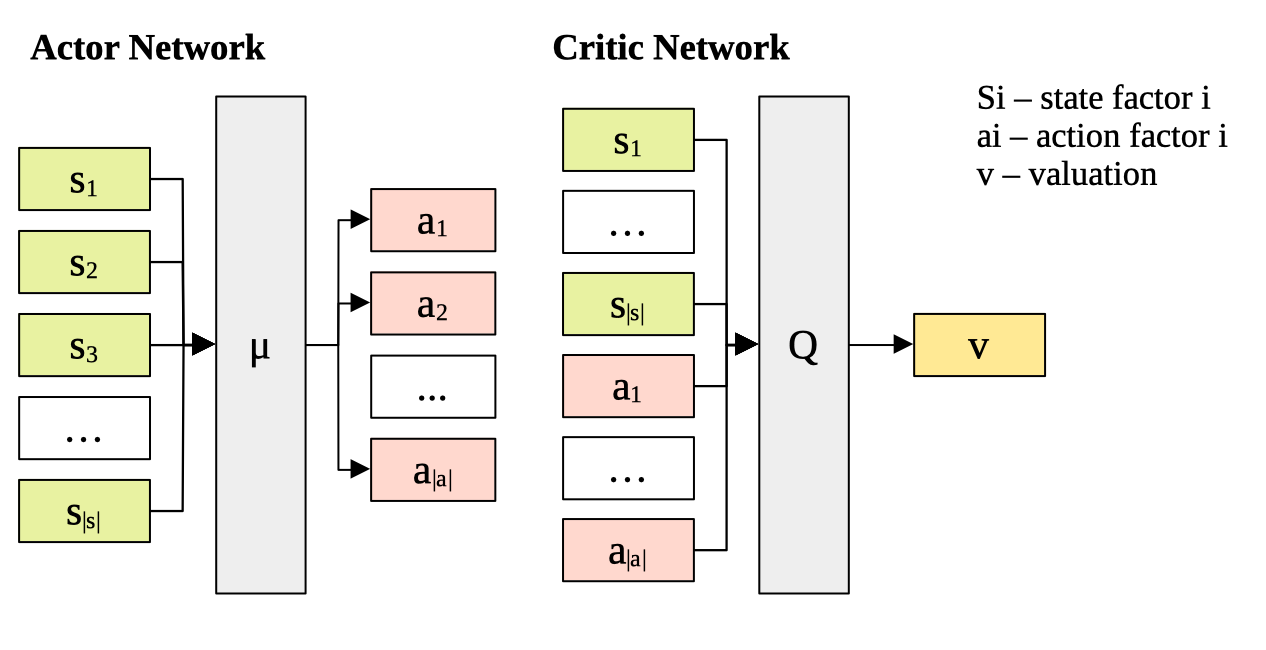
\includegraphics[width=.46\textwidth]{figure/ddqn1}}
    \hfill
    \subcaptionbox{Active-Target Pair}
    {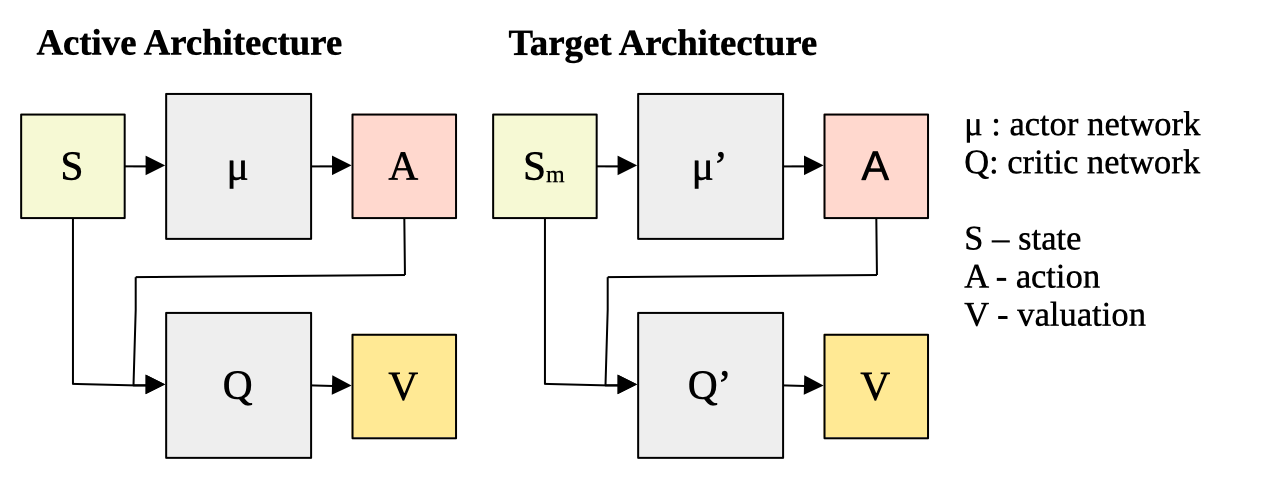
\includegraphics[width=.46\textwidth]{figure/ddqn2}}
    \caption{Diagram of (a) the actor-critic network layout 
    and (b) the active-target transfer learning air used by
    agents}
    \label{fig:farm_ddqn}
\end{figure}

\subsection{Agent Decision-Making}
\label{subsec:farm_methods_decisions}

In traditional agent-based models, agents make decisions according to
rule-based decision-policies or probabilistic methods.
In integrating machine learning,
agents instead make decisions according to an internal decision-policy
function $\pi(s)=a$ mapping the state of each agent to the potential actions 
that each agent can take.
In this approach, the decision-policy function is being approximated by
an artificial neural network (ANN), $\mu:S\rightarrow A$.
The input to this ANN is the state of the agent, vectorized as a 1-dimensional
array of length $W_S$.
The output of the ANN is a vector of length $W_A$ encoding the action that
the ANN has decided the agent should take.

Each time an agent needs to take an action,
it passes its current state through the network to generate an action.
It performs this action with some probability $1 - \epsilon$.
With probability $\epsilon$, the agent will instead take a random action.
This random action is used to encourage exploration of the state space
and to prevent the agent from getting stuck in a local optimum.

\subsection{Agent Learning}
\label{subsec:farm_methods_learning}

The policy evaluation network, $Q$, is updated using the Q-learning
update function (Eq~\ref{eq:q_update}), where
$S_t$ and $A_t$ are the state and selected action at time $t$,
$\alpha$ is the learning rate,
and the target $Y_t^{DDQN}$ is defined as a function of the
state, action, and received reward value $R_t$ (Eq~\ref{eq:q_target}).

\begin{equation}
\label{eq:q_update}
    \forall \theta \in \Theta_Q \left[
    \theta_{t+1} = \theta_t + \alpha\left(
    Y_t^{DDQN} - Q(S_t, A_t)
    \right)
    \nabla_{\theta_t}Q(S_t,A_t)
    \right]
\end{equation}

\begin{equation}
\label{eq:q_target}
    Y^{DDQN} = 
        R_{t+1}
        + \gamma Q'\left(S_{t+1},\argmax{a}{Q(S_{t+1}, a}\right)
\end{equation}

Because the networks in this system update are training
using experience replay, the argmax term present in 
Equation~\ref{eq:q_target} is replaced with the output of the 
target actor~$\mu'(S_{t+1})$ as part of a batch update of 
batch size~$B$.
The actor network~$\mu$ also updates from the selected
experience batch, using policy gradient with regard to
the resulting valuations provided by $Q$.

The target architecture initially has the same weights as
the main architecture, at the end of each training episode,
weights from the main architecture are copied to the target
architecture according to the transfer learning function
(Eq~\ref{eq:tr}).

\begin{equation}
    \label{eq:tr}
    \forall\theta_i'\in\Theta'\left[
        \theta_i'\leftarrow\tau\theta_i+\left(1-\tau\right)\theta_i',
        \tau \ll 1
    \right]
\end{equation}


\subsection{Agent Memory}
\label{subsec:farm_methods_memory}

Agents in the model store a history of their past experience as
a series of state transition records $(s_t,a_t,r_t,s_{t+1})$.
These records are stored in a memory buffer $B$ of fixed length $N$.
When the memory buffer is full, new records overwrite the oldest records in
the buffer.
The memory buffer is used to train the agent's decision-policy and valuation.

Additionally,
agents have a built-in `forgetfulness factor', $F$,
which has been incorporated in an attempt to capture some of the behavior
patterns of human actors with imperfect memory.
This factor is a real number between 0 and 1 and is used to linearly scale the
amount of noise that is introduced into the memory record as the record
ages within a run.
An agent with $F=0$ will have perfect recall of its entire state transition
history, whereas an agent with $F=1$ will have perfect recall of its most
recent state transition with actions taken in the distant past being
completely forgotten (noise term of equal range as actual term).

\begin{algorithmic}
\ForAll{agents in each time step}
\State With probability $\epsilon$ select random action $A_t$
\State otherwise select action $A_t \gets \mu(S_t)$
\State Execute $A_t$ and observe reward $R_t$ and next state $S_{t+1}$
\State Push transition record to memory $M[m]\gets (S_t, A_t, R_t, S_{t+1})$
\State Select random minibatch $B$ of $N$ transitions from memory $M$
\If{Agent is forgetful, $F > 0$}
\State Introduce random noise to transition record proportional to the
\State temporal distance to transition $(m-t)$ and agent forgetfulness $F$
\EndIf
\State Perform Q-learning update via action replay
\State Perform $\mu$ update via policy gradient
\EndFor
\end{algorithmic}


\section{Experimental Design}
\label{sec:farm_ex}

\subsection{Model Overview}

In order to test this modeling methodology for the integration
of deep reinforcement machine learning into an agent-based model,
an experimental ABM was developed.
This ABM is a model of a multi-agent of agricultural decision-makers
and how their behavior may change in response to external stimuli.
The real-world basis for this model is a study area in the
Missisquoi Bay Area of the Lake Champlain Basin of Vermont,
and the model is designed to represent the agricultural decision-making
processes of farmers in this area ---
in particular, decisions pertaining to agricultural productivity
and the adoption or rejection of agricultural best management practices~(BMPs).

\subsubsection{Agents}

There are two types of agents present in this model --- 480 farmer agents, 
corresponding to the 480 agriculturally-zoned land parcels in the
Missisquoi Bay Area, 
and a single regulatory agent.
All agents in the model contain some internal information 
about their current state and history,
a set of state-transition memories used to learn from experience,
and a set of neural networks used to drive agent decision-making. 
As the agents make decisions over time, 
they gradually learn the correlation between 
the actions they take from each state using deep reinforcement machine 
learning.

The 480 agricultural agents model the behavior of farmers, herders,
and other kinds of agricultural land managers within the study area.
They make annual decisions about their farming practices, 
including whether they should change production in 
one of the four modeled agricultural industries 
(beef, dairy, corn, and hay) and whether they should implement 
an agricultural best management practice (BMP) to reduce 
phosphorus runoff on their land.

The state properties and variables that make up each agricultural agent
are listed in Table~\ref{tab:farm_state_farm}.
The initialization of these values is detailed in
Section~\ref{sec:farmer_init}.

Conditions that factor in as components of a farmer agent's state 
include the total land area the agent has devoted to cropland or pasture; 
the productivity of the agent in each of the four modeled agricultural 
industries along with their associated phosphorus byproduct productivity; 
an 5-year history of the farm's profitability, storm losses, and BMP usage; 
and similar historical information from the agent's k-nearest neighboring
farmer agents.

This subset of state factors is summarized along with those of
the regulatory agent in Table~\ref{tab:farm_agents_states}.
For the farmer agents, these break down into a few main groups:
information about their own land cover,
information about their productivity in the given time-step,
a 5-year history of their own experiences,
and historical information from their 5-nearest neighbors.

\begin{longtable}{lll}
\caption{Table of the state properties of agricultural agents and their
associated data type for agricultural agents in the agricultural model.} 
\label{tab:farm_state_farm} \\
\hline \hline
Name & Description & Data Type \\
\hline
\endfirsthead
\caption[]{(continued...)}\\
\hline\hline
Name & Description & Data Type \\
\hline\endhead
\hline
\endfoot
\hline
\endlastfoot
Agent ID & Unique identifier for this agent & \tt{uint} \\
Agent Status && \tt{enum\{3\}} \\
Land Parcel Data \\
\multicolumn{1}{r}{Crop Land Area $A_c$} & Land devoted to growing crops (sq km) & \tt{float} \\
\multicolumn{1}{r}{Pasture Land Area $A_p$} & Land devoted to grazing animals (sq km) & \tt{float} \\
\multicolumn{1}{r}{Total Land Area $A_{tot}$} & Total land in parcel (sq km) & \tt{float} \\
Productivity \\
\multicolumn{1}{r}{Corn $p_c$} & Corn production factor & \tt{float} \\
\multicolumn{1}{r}{Hay $p_h$} & Hay production factor & \tt{float} \\
\multicolumn{1}{r}{Beef $p_b$} & Beef production factor & \tt{float} \\
\multicolumn{1}{r}{Dairy $p_d$} & Dairy production factor & \tt{float} \\
\multicolumn{1}{r}{Phosphorous $p_{p,x}$} & Phosphorus production factor & \tt{float} \\
Cows Owned $C$ & Number of cows on farm & \tt{uint} \\
Financial History \\
\multicolumn{1}{r}{Real Net} & What was net profit over last 5 years & \tt{float[5]} \\
\multicolumn{1}{r}{Expected Net} & What was expected profit for last 5 years
& \tt{float[5]} \\
Extreme Event History & Extreme event presence over past 5 years & \tt{uint[5]} \\
BMP Usage History $B$& Did farm use BMP in last 5 years & \tt{bool[5]} \\
Neighbors & References to neighboring agents & \tt{farmer*[5]} \\
Neural Networks && \\
\multicolumn{1}{r}{Actor Network $\mu$} & Network Weights & \tt{float[l][w]} \\
\multicolumn{1}{r}{Critic Network $Q$} & Network Weights & \tt{float[L][W]} \\
\multicolumn{1}{r}{Target Network $\mu'$} & Network Weights & \tt{float[l][w]} \\
\multicolumn{1}{r}{Target Network $Q'$} & Network Weights & \tt{float[L][W]} \\
Memory Bank && \tt{float[M*R]} \\
Memory Buffer && \tt{float[B*R]} \\
\end{longtable}

The actions that the farmer agents can take are listed in
Table~\ref{tab:farm_action_farm}.
These actions are divided into two main categories:
the action of choosing to adopt or not adopt a BMP for their farm,
and adjusting the farm's productivity in one of the four agricultural
sectors.

\begin{longtable}{p{.4\textwidth}p{.5\textwidth}}
\caption{A summary of the actions being select by the agricultural
agents in the agricultural model.}
\label{tab:farm_action_farm} \\ \hline \hline
Group & Action \\ \hline
\endfirsthead
\hline\endfoot
\hline\endlastfoot
BMP Usage & Adopt BMP  \\
    & Don't Adopt BMP  \\
Corn Production & Increase by $[0, S^+_c)$  \\
    & Maintain  \\
    & Decrease by $[0, S^-_c)$  \\
Hay Production & Increase by $[0, S^+_h)$  \\
    & Maintain \\
    & Decrease by $[0, S^-_h)$  \\
Dairy Production & Increase by $[0, S^+_d)$  \\
    & Maintain  \\
    & Decrease by $[0, S^-_d)$  \\
Beef Production & Increase by $[0, S^+_b)$  \\
    & Maintain  \\
    & Decrease $[0, S^-_b)$  \\
\end{longtable}

The production factors are a scalar component of production
functions that have been calculated for the region and
calibrated for the years 2001--2040.
These functions are shown below for the production of corn (Eq~\ref{eq:fcorn}),
hay (Eq~\ref{eq:fhay}),
dairy (Eq~\ref{eq:fdairy}),
and beef (Eq~\ref{eq:fbeef}),
where $t$ is the modeled year.

\begin{equation}
\label{eq:fcorn}
    P_c(t) = p_c * A_c^b * 11.433\log{t} - 86.826
\end{equation}
\begin{equation}
\label{eq:fhay}
    P_h(t) = p_h * A_c^b * \SI{1e-32}{}\exp{0.0358t}
\end{equation}
\begin{equation}
\label{eq:fbeef}
    P_b(t) = p_b * A_p^b * \SI{2e-20}{}\exp{0.0234t}
\end{equation}
\begin{equation}
\label{eq:fdairy}
    P_d(t) = p_d * A_p^b * \SI{2e-9}\exp{0.0114t}
\end{equation}

The productivity of the agent is modified by
the application of the regulatory agent's regulations $G_1$ (Eq~\ref{eq:g1}) 
and $G_2$ (Eq~\ref{eq:g2})
and the amount of losses due to extreme weather events (Eq~\ref{eq:f_stormloss})
as a function of whether the BMP was used and whether the number
of extreme events that occurred within the given year exceeds the
expected threshold from the weather submodel.

\begin{equation}
\label{eq:f_stormloss}
\begin{array}{lllll}
    S(B, EE) & = & 1, & EE < N & \\
    S(B, EE) & = & 0.1, & EE \ge N, & \neg B \\
    S(B, EE) & = & (0.1 + 0.9 B_e), & EE \ge N, & B \\
\end{array} 
\end{equation}

The weather submodel would generate a number of rainfall events
for the study area every model year, according to a distribution
calibrated according to historical rainfall data for the region
from the years 1920--1980.
The number of weather events that were necessary to occur to
be considered an extreme event year was determined by
using peaks-over-threshold for the historical data. 

The reward function used for training the policies of the
farmer agents (Eq~\ref{eq:f_farmreward})
is defined by the ratio of the squared 
realized profits of a time-step (Eq~\ref{eq:f_netprofit})
and the expected profits at that time-step (Eq~\ref{eq:f_expprofit}),
translated from the range of all possible profits $(P_{\min}, P_{\max})$
to the range $(-1, 1)$.

\begin{equation}
\label{eq:f_netprofit}
    P_{net}(t) = \sum_x P_x(t) G_1(P_p, B, t) S(B, EE) + G_2(P_p, B, t)
\end{equation}

\begin{equation}
\label{eq:f_expprofit}
    P_{exp}(t) = \sum_x P_x(t) G_1(P_p, B, t) + G_2(P_p, B, t)
\end{equation}

\begin{equation}
\label{eq:f_farmreward}
    R_f(t) = 
    \frac{P_{net}(t)^2}{P_{exp}(t)} 
    : \left(P_{\min}, P_{\max}\right) \rightarrow \left(-1, 1\right)
\end{equation}

The one municipal regulatory agent is used to model a municipal 
government or regulatory agency's behavior managing agricultural 
practices on the landscape 
and the local environment and the policies that guide them. 
This agent acts more slowly than the agricultural agents, 
once every five time-steps, and decides if/how it should modify 
its incentive structure 
--- changing its taxation rate, the subsidization given to an agent 
adopting a BMP, and the phosphorus runoff threshold at which a penalty is 
applied.
The state properties of the regulatory agent are listed in
Table~\ref{tab:farm_state_reg},
and details on their initialization are included in
Section~\ref{sec:regulator_init}.

\begin{longtable}{lcll}
\caption{Table of the state properties of the regulatory agent and their associated data type
for the regulatory agent in the agricultural model.}
\label{tab:farm_state_reg} \\
\hline\hline
Name && Description & Data Type \\
\hline
\endfirsthead
\caption[]{(continued...)} \\
\hline\hline
Name && Description & Data Type \\
\hline
\endhead
\hline
\endfoot
Agent ID && & \tt{uint} \\
Aggregate Agent Data & & \\
\multicolumn{1}{r}{BMP Adoption} && & \tt{float[15]} \\
\multicolumn{1}{r}{Extreme Events} && & \tt{uint[15]} \\
\multicolumn{1}{r}{Financial History} && & \tt{float[15]} \\
\multicolumn{1}{r}{P Runoff History} && & \tt{float[15]} \\
Regulation Change Limit & $g$ & & \tt{float} \\
P Tax Rate & $T_p$ & & \tt{float} \\
P Tax Threshold & $P_t$ & & \tt{float} \\
BMP Subsidy Value & $S_b$ & & \tt{float} \\
Neural Networks && \\
\multicolumn{1}{r}{Actor Network} & $\mu$ & Network Weights & \tt{float[l][w]} \\
\multicolumn{1}{r}{Critic Network} & $Q$ & Network Weights & \tt{float[L][W]} \\
\multicolumn{1}{r}{Target Network} & $\mu'$ & Network Weights & \tt{float[l][w]} \\
\multicolumn{1}{r}{Target Network} & $Q'$ & Network Weights & \tt{float[L][W]} \\
Memory Bank &&& \tt{float[M*R]} \\
Memory Buffer &&& \tt{float[B*R]} \\
\end{longtable}

The components of actions that the regulatory agent can take
are listed in Table~\ref{tab:farm_action_reg}
The phosphorus threshold adjustment action is notably implemented
differently in that it is a single value which is having the sign taken
to determine the direction of the adjustment.

% TABLE -- ACTIONS
\begin{table}
    \caption{A summary of the action factors being used to drive agent
    decision-making for both types of agent present in the model.}
    \label{tab:farm_action_reg}
    \begin{tabularx}{\linewidth}{lX}
        \emph{Regulator Agent} \\
        \hline
        \hline
        Group & Action  \\
        \hline
        Tax Rate & Increase by $[0, T^+_g)$ \\
        & Decrease by $[0, T^-_g)$ \\
        BMP Subsidy & Provide/Increase \\
        & Remove/Decrease  \\
        Phosphorous Threshold$\star$ & Scale  \\
        \hline
    \end{tabularx}
\end{table}

% TABLE -- STATES
\begin{table}[p]
    \centering
    \caption{A summary of the state factors being used as input to the
    agents' ANNs.}
    \label{tab:farm_agents_states}
    \begin{tabularx}{\linewidth}{XXl}
        \emph{Farmer Agent} \\
        \hline\hline
        Group & Description & Detail \\
        \hline
        Land Cover & Cropland & Normalized Area (sq m) \\
        & Pasture & Normalized Area (sq m) \\
        Productivity & Corn & See \ref{app:farm} \\
        & Hay \\
        & Dairy \\
        & Beef \\
        History (5-year) & Extreme Event Record & Occurrence \\
        & Financial Record & \ref{app:farm} \\
        & BMP Adoption Record & \\
        Network Information & Financials & Losses (1-year, 5-year) \\
        & BMP Adoption & Usage (1-year, 5-year) \\
        \hline \\[1.0em]
        \emph{Regulator Agent} \\
        \hline
        \hline
        Group & Description & \\
        \hline
        Aggregate Data & \multicolumn{2}{l}{BMP Adoption} \\
        & Financials & Net Profits, Losses \\
        & \multicolumn{2}{l}{P Runoff} \\
        History & Extreme Event Record & 5-year, 15-year \\
        & \multicolumn{2}{l}{BMP Adoption} \\
        & Financials & Net Profits, Losses \\
        & \multicolumn{2}{l}{P Runoff} \\
        \hline
    \end{tabularx}
\end{table}


The results of taking these actions is a shift in the regulatory
parameters of the system as shown in the set of equations below
(Eq~\ref{eq:reg_shift}).

\begin{equation}
    \label{eq:reg_shift}
    \begin{array}{l|lcl}
    a_0 & T_{p, t+1} & = & T_{p, t} 
        + \min_{\ge0}\left(T_p^+, \norm\left(\delta T_p, g+k\right)\right) \\
    a_1 & T_{p, t+1} & = & T_{p, t} 
        - \min_{\ge0}\left(T_p^-, \norm\left(\delta T_p, g+k\right)\right) \\
    a_2 & S_{b, t+1} & = & T_{p, t} 
        + \min_{\ge0}\left(S_b^+, \norm\left(\delta S_b, g+k\right)\right) \\
    a_3 & S_{b, t+1} & = & T_{p, t} 
        - \min_{\ge0}\left(S_b^-, \norm\left(\delta S_b, g+k\right)\right) \\
    a_4 & P_{t,t+1} & = & P_{t, t} 
        + \text{signum}\left(a_4\right) \\
    \end{array}
\end{equation}

The parameter changes impact the incentive structures
provided by the phosphorus taxing function, $G_1$,
shown in Equation~\ref{eq:g1},
and the BMP subsidization function, $G_2$,
shown in Equation~\ref{eq:g2}.

\begin{equation}
\label{eq:g1}
    G_1(P, B, t) = \left\{
    \begin{array}{ll}
        T_p & P_p \ge P_t \\
        1 & P_p < P_t \\
    \end{array}
    \right.
\end{equation}

\begin{equation}
\label{eq:g2}
    G_2(P, B, t) = \left\{
    \begin{array}{ll}
    S_b & B \\
    0 & \neg{B} \\
    \end{array}
    \right.
\end{equation}

The goal of the regulator agent is to minimize the aggregate phosphorous
output and storm loss of all agricultural agents,
$R_r = \left<W_p\sum_fP_{p,f}(t), W_l\sum_fl_f\right>$,
where $W_p$ and $W_l$ are normalizing weights on the component
inverse reward signals so that they vary along ranges of similar magnitude.

The parameters for agent learning for both agent types are summarized in
Table~\ref{tab:farmsanns}.

% TABLE -- ANN PARAMS
\begin{table}[h]
\centering
\caption{Network parameters for the ANNs used by agents in each class
    for the land cover model}
\label{tab:farmsanns}
    \begin{tabular}{@{\extracolsep{4pt}}lp{.15\linewidth}>{\centering}p{.15\linewidth}>{\centering}p{.15\linewidth}cc@{}}
\hline
\hline
\multirow{2}{*}{Parameter} 
    & \multicolumn{2}{c}{Agricultural} 
    & \multicolumn{2}{c}{Regulatory} \\
    \cline{2-3}\cline{4-5}
 & $\mu$ & $Q$ & $\mu$ & $Q$ \\
\hline
Input Nodes  & 15 & 32 & 10 & 15 \\
Inner Layers  & 4 & 3 & 4 & 3  \\
Inner Nodes  & 10 & 16 & 7 & 7 \\
Output Nodes  & 17 & 1 & 5 & 1 \\ 
Connectivity & \multicolumn{4}{c}{--- Full ---} \\
Activation Function & \multicolumn{4}{c}{--- ReLU ---} \\
Output Activation & 5-hot & Linear & 2-hot + 1-Signum & Linear \\
\hline
\end{tabular}
\end{table}



\subsubsection{Model Hyperparameters}

Preliminary model runs were conducted to determine the optimal values for
the hyperparameters for machine learning within the model.
The learning hyperparameters that were varied in these preliminary runs were
the number of training episodes,
the number of steps between target network updates,
the number of inner layers in the neural networks,
the number of neurons in each of those inner layer,
the learning rate,
and the batch size.
The learning hyperparameters that were held constant were
the exploration rate at $\epsilon = 0.1$,
the discount factor at $\gamma = 0.99$,
the learning transfer rate at $\tau = 0.001$,
the number of steps within a training episode at $N = 40$,
the relay memory size at $M = 10000$.

\begin{longtable}{lcll}
\caption{Hyperparameters and their associated values with source or
rationale, if applicable, for the agricultural land-use model.}
\label{tab:farm_hyper} \\ \hline \hline
Parameter && Value & Source/Rationale \\ \hline
\endfirsthead
\caption[]{(continued...)}\\ \hline \hline
Parameter && Value & Source/Rationale \\ \hline
\endhead
\hline\endfoot
Learning Rate & $\alpha$ & 0.00025 & \\
Exploration Rate & $\epsilon$ & 0.1 & \\
Discount Factor & $\gamma$ & 0.99 & \\
Transfer Rate & $\tau$ & 0.001 & \cite{ddqn16} \\
Relay Memory Size & $M$ & 10000 & \cite{ddqn16} \\
Number of Episodes & $N$ & 1000 & \\
Number of Steps per Episode & $T$ & 40 & Economic production function limitation \\
\end{longtable}



\subsection{Experimental Setup}
\label{subsec:farm_ex_setu}

The model was run for a variety of scenarios.
All scenarios tested the variables $BMP_e$, $\Delta EE$,
and $g$.
There were two classes of test:
tests with agents with uniform memory accuracy (Table~\ref{tab:farm_ex_ar})
and tests with agents with heterogeneous memory accuracy
(Table~\ref{tab:farm_ex_mix}).

BMP Efficacy ($B_e$) was varied from 0.0 to 1.0 in increments of 0.1.
This parameter represents the effectiveness of BMPs in reducing nutrient
loading from agricultural fields.
A value of 0.0 indicates that BMPs have no effect on nutrient loading,
while a value of 1.0 indicates that BMPs completely eliminate nutrient loading.
This parameter was varied in order to determine the effect of BMP efficacy
on the behavior of the system.

Change in weather event frequency ($\Delta EE$) was varied from -0.2
to 0.2 in increments of 0.05.
This parameter represents the change in the frequency of extreme weather
events, such as heavy rainfall, that may be induced by climate change
compared to a historical baseline, so in cases where $\Delta EE = 0.2$,
the expected number of extreme rainfall events that are going to
occur will be 1.2 times the expected number of extreme rainfall events
according to the baseline.

The regulation change limiter ($g$) represents the maximum rate at which
the regulatory agent will adjust the regulatory environment.
Three values were tested: an aggressive limit ($g=0.2$),
a moderate limit ($g=0.05$), and
a restrictive case ($g=0$) for testing the model's ability to
operate in a static regulatory environment.
This value alters the width of the distribution that the regulatory
parameters, $T_p$ and $S_b$, are adjusted by.

The impact of agent memory accuracy was tested for two types of agent
populations.
In uniform agent populations, all agents had the same memory recall
accuracy ($F$), where $F$ is the probability that a memory will be
recalled correctly.
In heterogeneous agent populations, agents had different memory recall
accuracy, 
where a proportion of agents ($P$) had accuracy $F=1$
and all other agents ($1-P$) had accuracy $F=0$.

% TABLE - UNIFORM EX
\begin{table}
\centering
\caption{Table listing experimental parameters for uniform population runs}
\label{tab:farm_ex_ar}
\begin{tabular}{lll}
\hline
Variable & & Values \\
\hline
BMP Efficacy & $B_e$ & 0, 0.1, 0.2, 0.3, 0.4, 0.5, 0.6, 0.7, 0.8, 0.9, 1.0 \\
Change in Event Frequency & $\Delta EE$
    & -0.2, -0.15, -0.1, -0.05, 0.0, 0.05, 0.1, 0.15, 0.2 \\
Regulation Change Limiter & $g$
    & 0, 0.05, 0.2 \\
Forgetfulness Factor & $F$ & 0, 0.25, 0.5, 0.75, 1 \\
\hline
\end{tabular}
\end{table}

% TABLE - MIXED EX
\begin{table}
\centering
\caption{Table listing experimental parameters for mixed population runs}
\label{tab:farm_ex_mix}
\begin{tabular}{lll}
\hline
Variable & & Values \\
\hline
BMP Efficacy & $B_e$ & 0, 0.1, 0.2, 0.3, 0.4, 0.5, 0.6, 0.7, 0.8, 0.9, 1.0 \\
Change in Event Frequency & $\Delta EE$
    & -0.2, -0.15, -0.1, -0.05, 0.0, 0.05, 0.1, 0.15, 0.2 \\
Regulation Change Limiter & $g$
    & 0, 0.05, 0.2 \\
Population Mixing & $P$ & 0.25, 0.5, 0.75 \\
\hline
\end{tabular}
\end{table}

\section{Results}
\label{sec:farm_results}

\subsection{Model Performance}
\label{subsec:farm_results_robust}

For each model parameterization,
agents were trained for 1000 training episodes.
If more than 10\%  of the agents ($n=48$) in the model failed to converge
to a stable policy within 1000 training episodes, the model was discarded 
and retrained; however, this occurred in less than 2\% of model runs.
A plot showing the distribution of number of agents which converged
across model parameterizations is shown in Figure~\ref{fig:farm_sfc}.

\begin{figure}
\centering
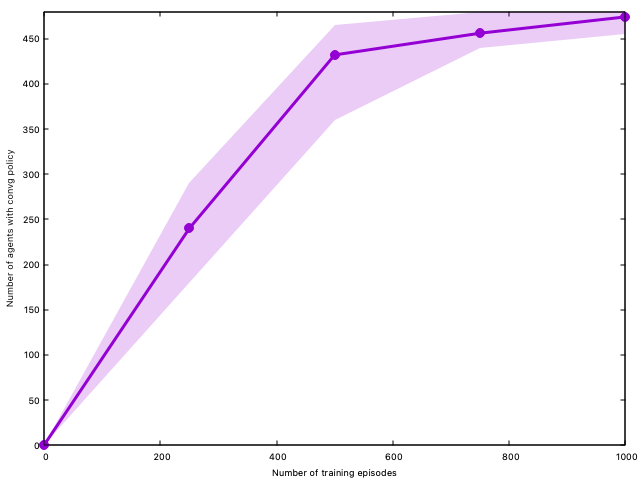
\includegraphics[width=.4\textwidth]{figure/sfc}
\caption{Plot of the number of agents that converged to a stable policy
    for each parameterization of the model}
\label{fig:farm_sfc}
\end{figure}

In this training,
an agent's networks were considered to have converged if after 50
initial training episodes, 
the net change in the weights of the network during a transfer learning step
was less than $10^{-5}$.
This threshold was chosen to be small enough to ensure that the networks
had reached some stable policy, but large enough to avoid overfitting.

Models which were successfully trained and passed through this screening
were then run for 40 testing runs.
Within this section,
some results have been omitted for readability.
A listing of results and their associated model parameterizations can be found in
Appendix~\ref{app:results}.

\begin{figure}
\centering
    \subcaptionbox{Initial State (y=2001)}{
        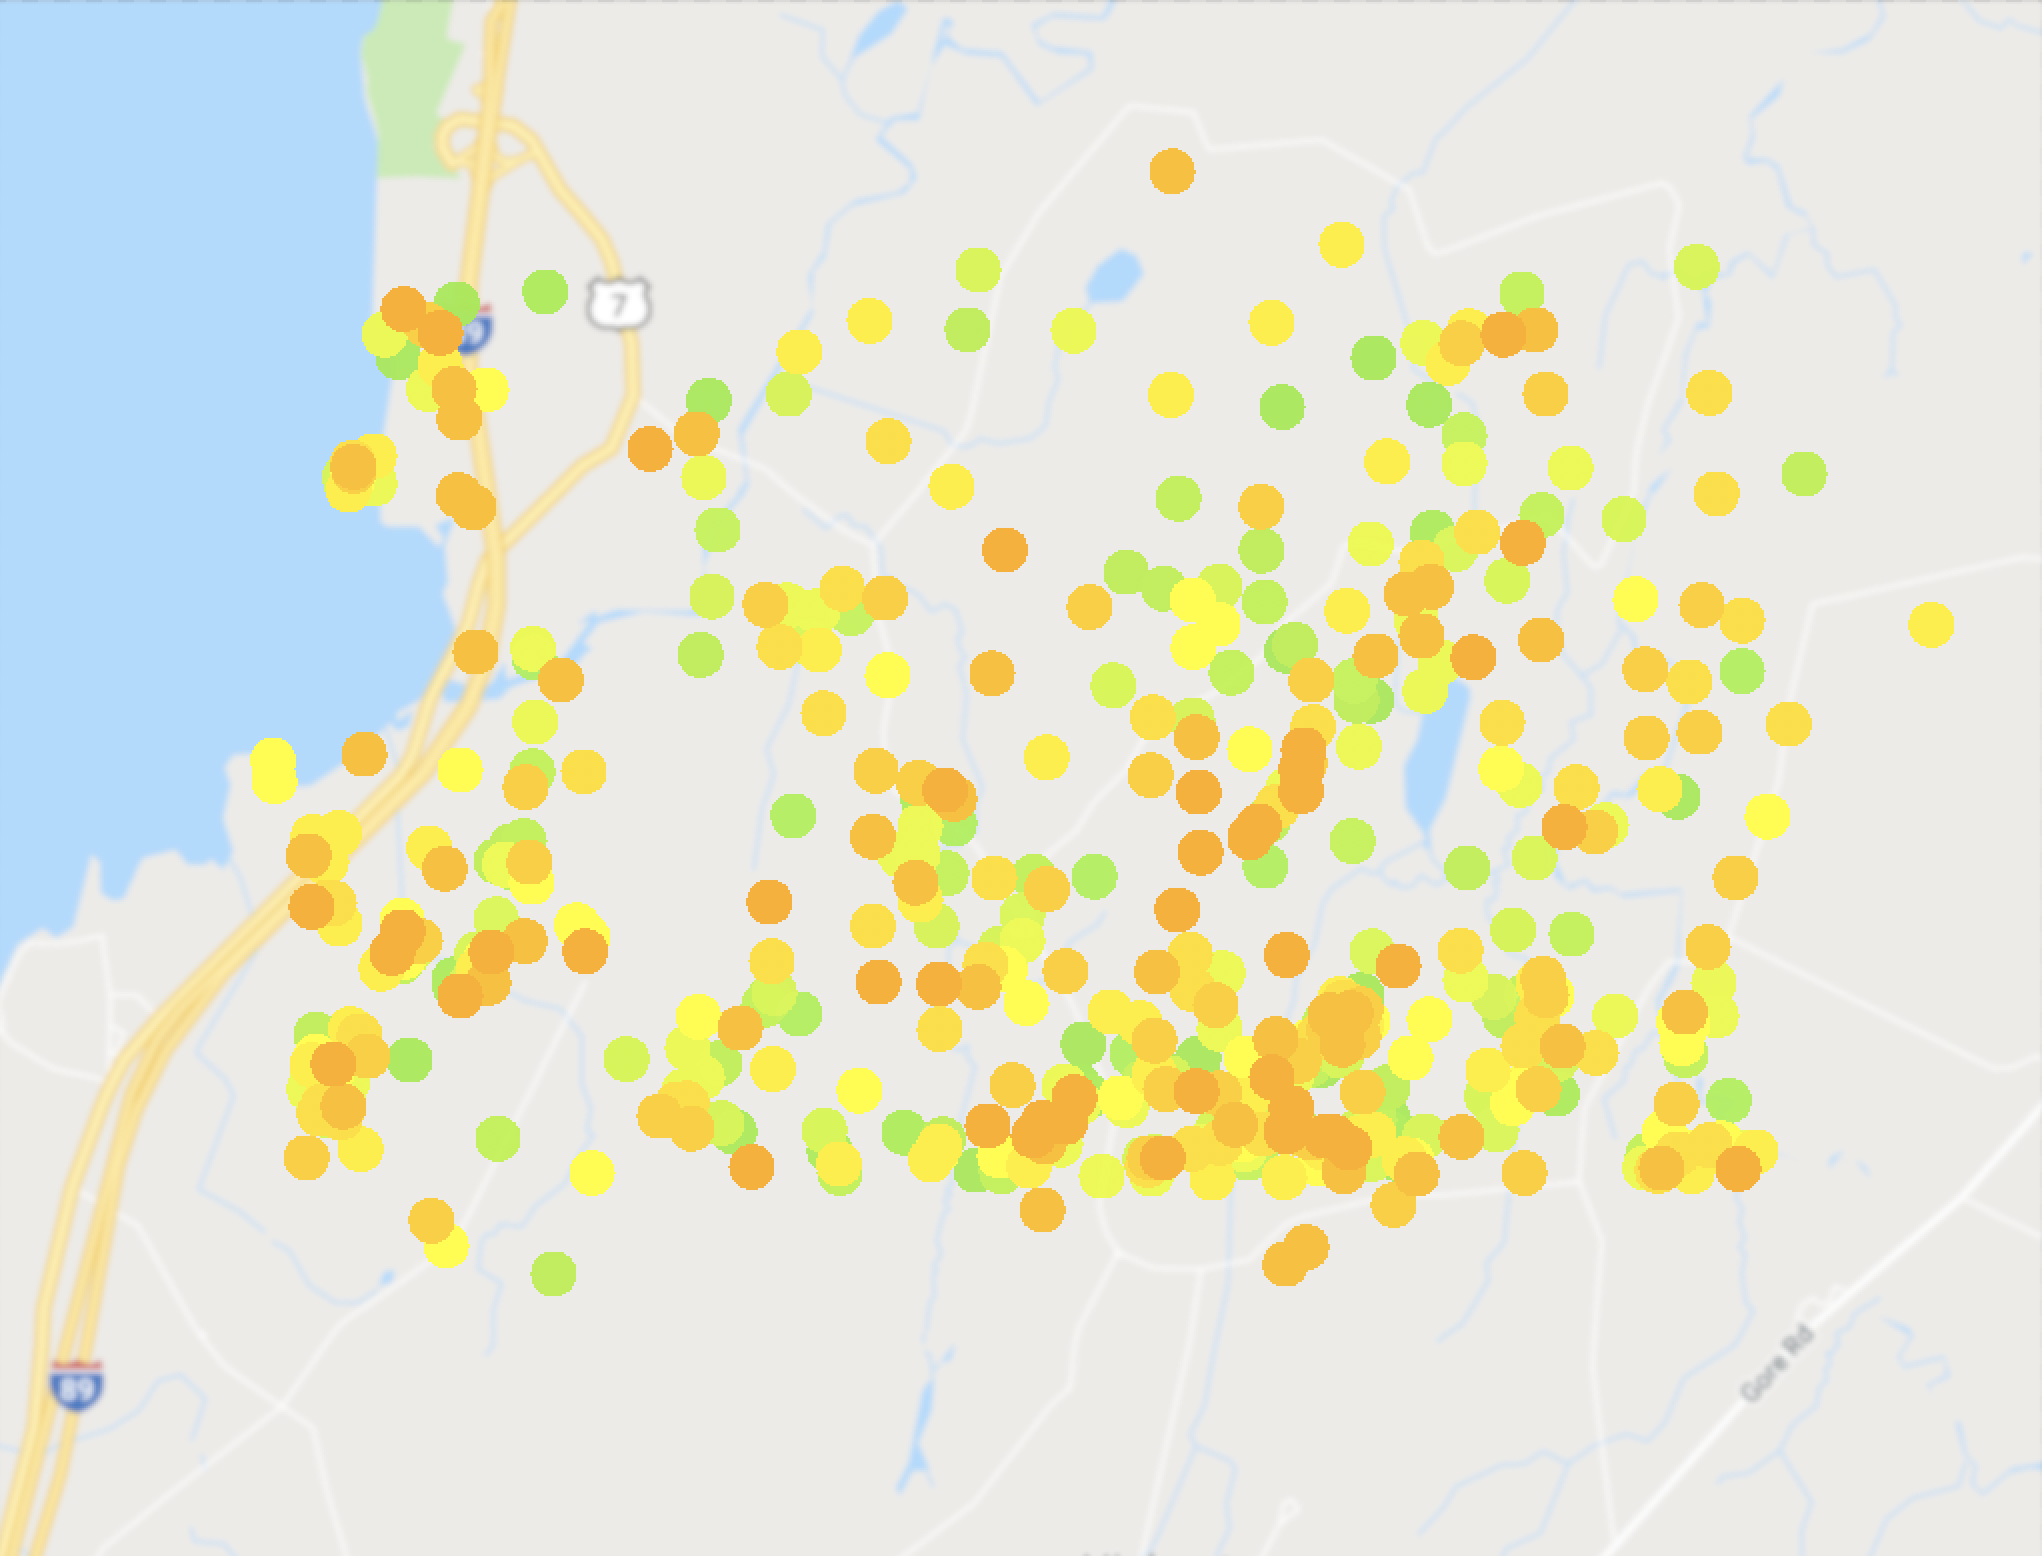
\includegraphics[width=0.3\linewidth]{figure/farm-sample-2001}
    }
    \hfill
    \subcaptionbox{End State (y=2040, g=0.05, $\Delta EE=0$)}{
        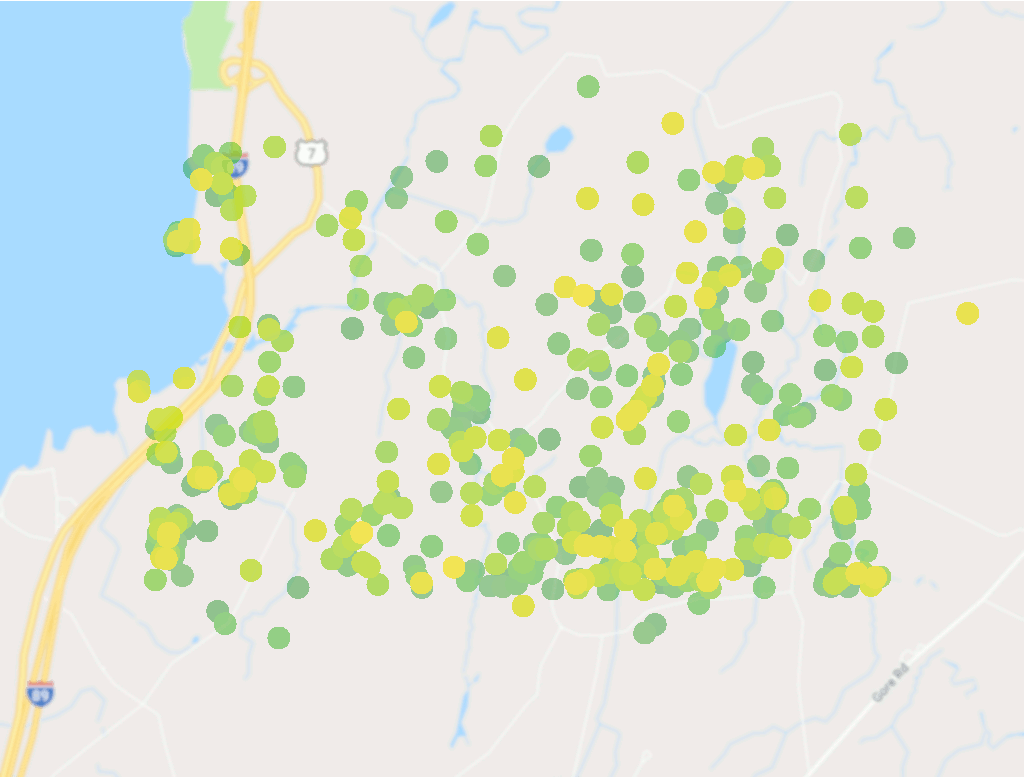
\includegraphics[width=0.3\linewidth]{figure/farm-sample-2040-1}
    }
    \hfill
    \subcaptionbox{End State (y=2040, g=0.2, $\Delta EE=0.2$)}{
        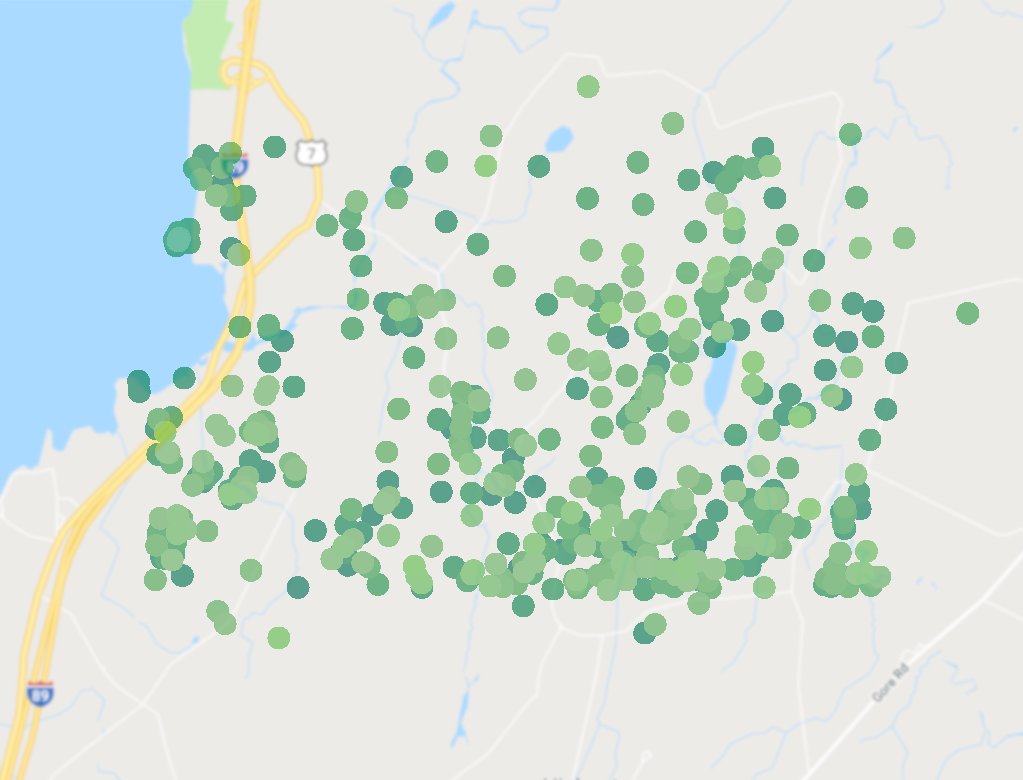
\includegraphics[width=.3\linewidth]{figure/farm-sample-2040-2}
    }
    \caption{Sample model output showing the change in BMP adoption likelihood
    from a characteristic initial model state (a) to a characteristic end states
    for (b)
    a model run with the parameterization ($g=0.05$, $\Delta EE=0$),
    and (c)
    a model run with the parameterization ($g=0.20$, $\Delta EE=0.2$).
    The color of each dot represents the likelihood that the agent will adopt
    BMPs, with green indicating a high likelihood and red indicating a low
    likelihood.}
    \label{fig:farm_mas}
\end{figure}

\subsection{Agent Behavior}
\label{subsec:farm_results_agents}

\subsubsection{Uniform Population Runs}

For model parameterizations with uniform agent populations,
the proportion of agents which adopted a BMP in each testing model run
was recorded and used to generate a distribution of BMP adoption rates
for each parameterization.
Summaries of the results of these runs are shown
in Figure~\ref{fig:farm_res_g00} for the case where the regulation change
threshold ($g$) was set to 0.0,
Figure~\ref{fig:farm_res_g05} for when $g$ was set to 0.05, and 
Figure~\ref{fig:farm_res_g20} for when $g$ was set to 0.2.

\begin{figure}[p]
    \subcaptionbox{$F=0$}{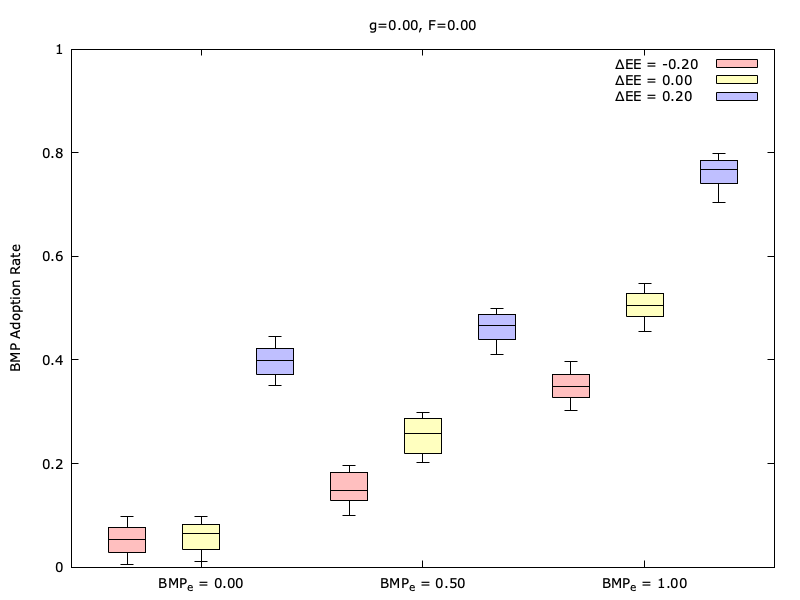
\includegraphics[width=.3\textwidth]{figure/g0F0}}
    \hfill
    \subcaptionbox{$F=0.5$}{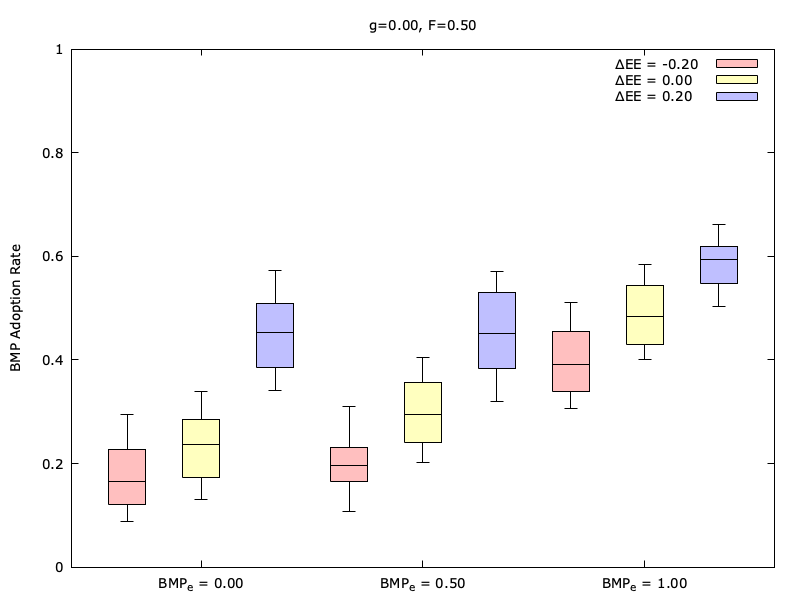
\includegraphics[width=.3\textwidth]{figure/g0F05}}
    \hfill
    \subcaptionbox{$F=1.0$}{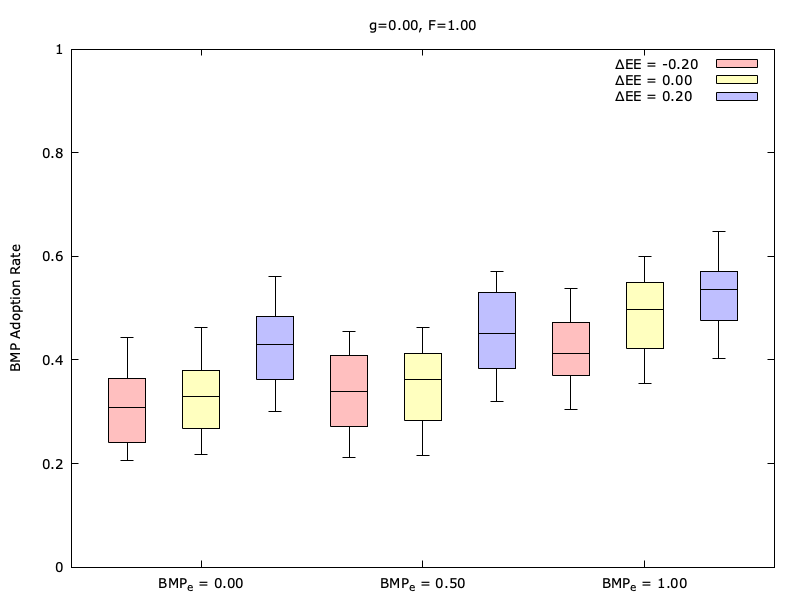
\includegraphics[width=.3\textwidth]{figure/g0F10}}
    \caption{Distribution of mean BMP adoption rate for uniform population
        runs of the agricultural land use model, where $g=0.0$,
        for (a) $F=0$, (b) $F=0.5$, and (c) $F=1.0$}
    \label{fig:farm_res_g00}
\end{figure}

\begin{figure}[p]
    \subcaptionbox{$F=0$}{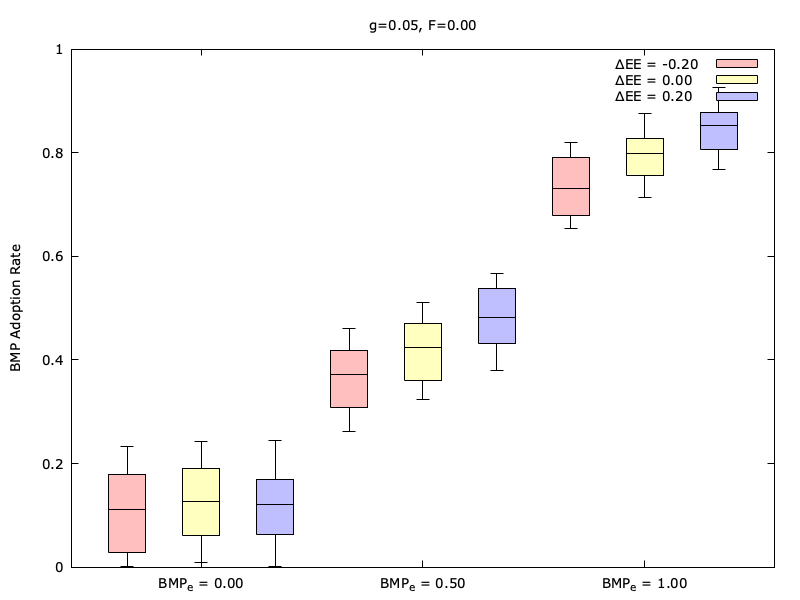
\includegraphics[width=.3\textwidth]{figure/g05F0}}
    \hfill
    \subcaptionbox{$F=0.5$}{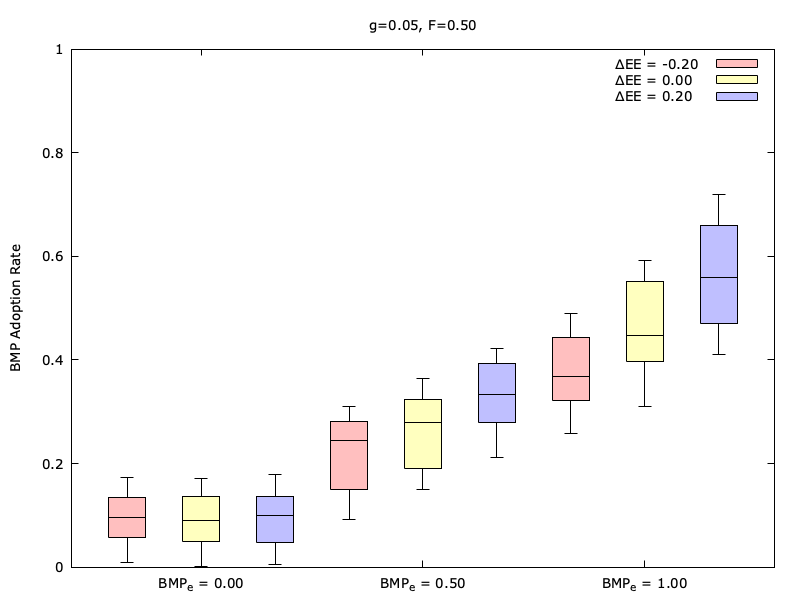
\includegraphics[width=.3\textwidth]{figure/g05F5}}
    \hfill
    \subcaptionbox{$F=1.0$}{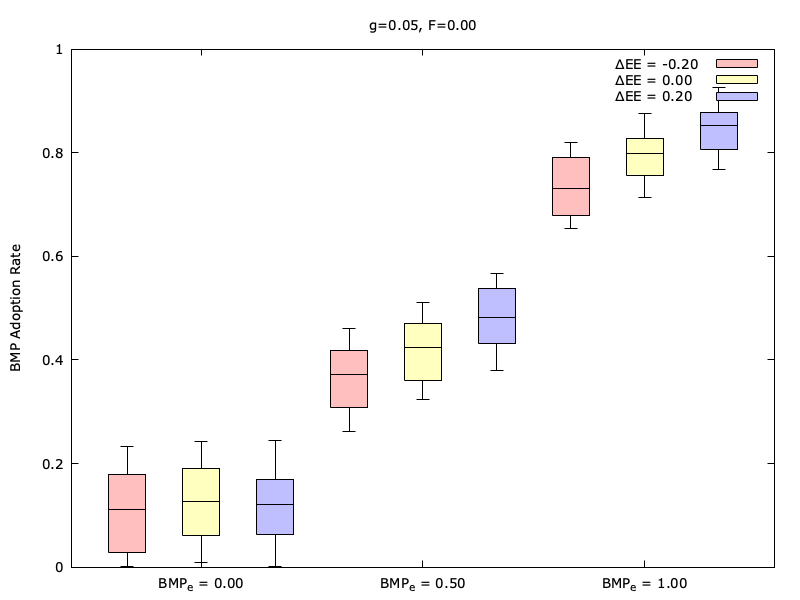
\includegraphics[width=.3\textwidth]{figure/g05F0}}
    \caption{Distribution of mean BMP adoption rate for uniform population
        runs of the agricultural land use model, where $g=0.05$,
        for (a) $F=0$, (b) $F=0.5$, and (c) $F=1.0$}
    \label{fig:farm_res_g05}
\end{figure}

\begin{figure}[p]
    \subcaptionbox{$F=0$}{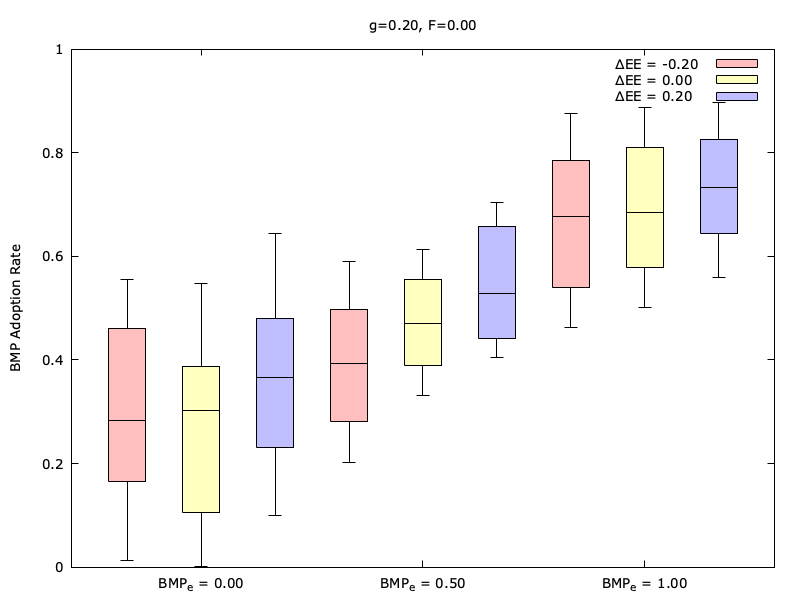
\includegraphics[width=.3\textwidth]{figure/g20F0}}
    \hfill
    \subcaptionbox{$F=0.5$}{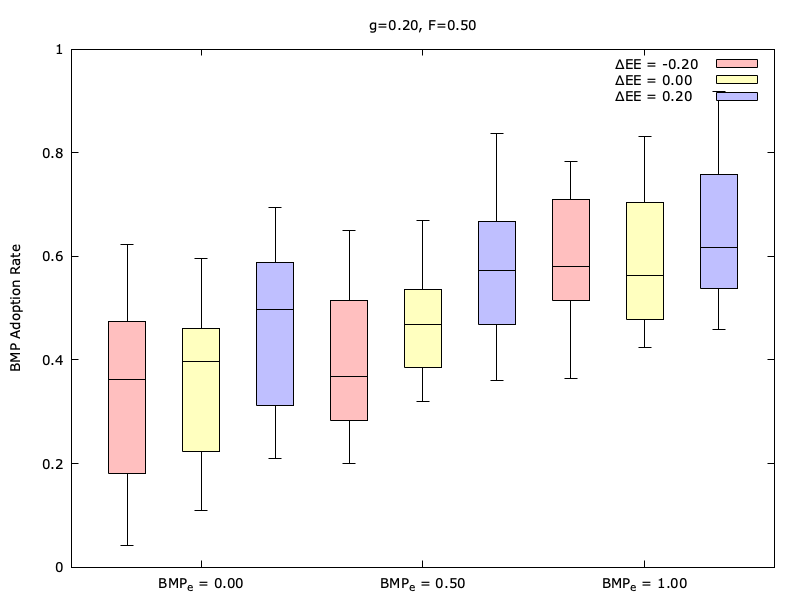
\includegraphics[width=.3\textwidth]{figure/g20F05}}
    \hfill
    \subcaptionbox{$F=1.0$}{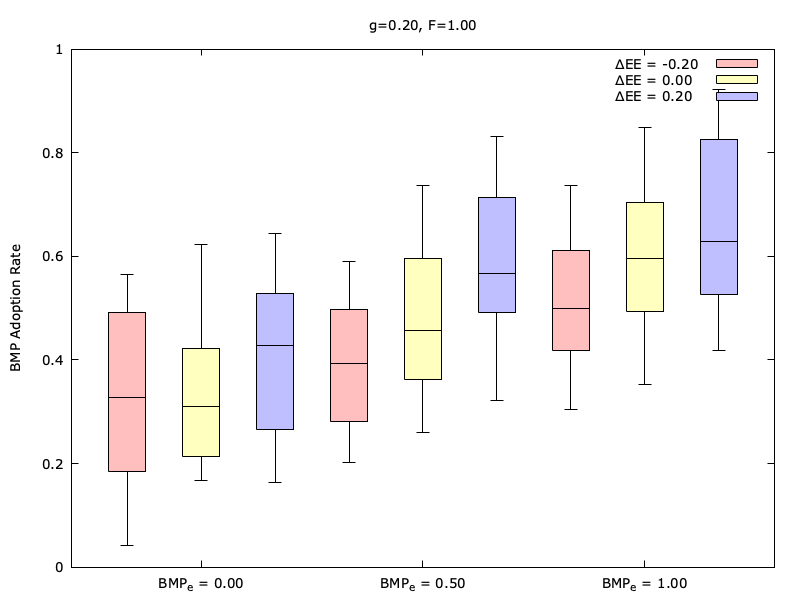
\includegraphics[width=.3\textwidth]{figure/g20F10}}
    \caption{Distribution of mean BMP adoption rate for uniform population
        runs of the agricultural land use model, where $g=0.2$,
        for (a) $F=0$, (b) $F=0.5$, and (c) $F=1.0$}
    \label{fig:farm_res_g20}
\end{figure}

\subsubsection{Mixed Population Runs}

For model parameterizations with mixed agent populations,
agents were divided into three groups:
group 1, where $F=0$ for the agent and all neighbors,
group 2, where $F=1$ for the agent and all neighbors, and
group 3, for agents with neighbors where $F=0$ and $F=1$. 
The proportion of agents in each group which adopted a BMP in each testing
model run was recorded and used to generate a distribution of BMP adoption
rates for each parameterization.
Results of one set of parameterizations of these runs are shown
in Figure~\ref{fig:farm_res_mix0} where $g=0$, $\Delta EE=0$.

\begin{figure}
    \subcaptionbox{$P=0.25$}{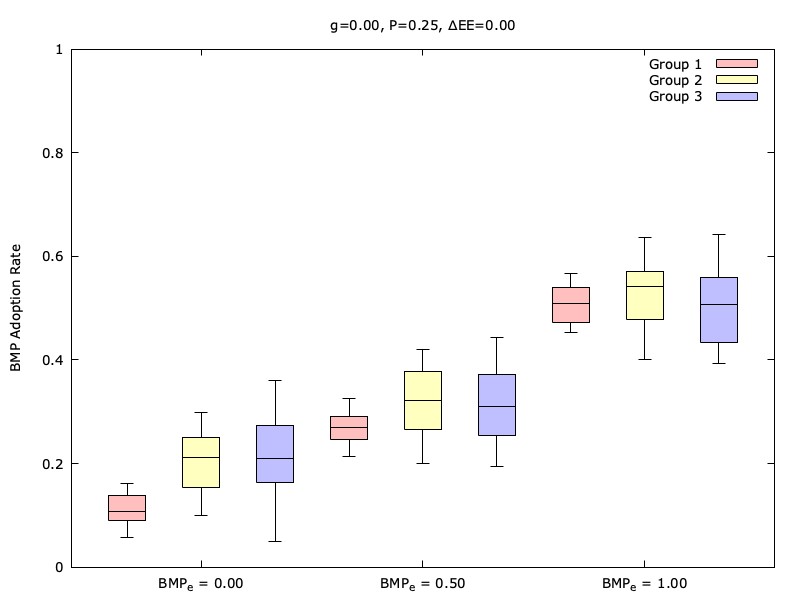
\includegraphics[width=.3\textwidth]{figure/g0P25}}
    \hfill
    \subcaptionbox{$P=0.5$}{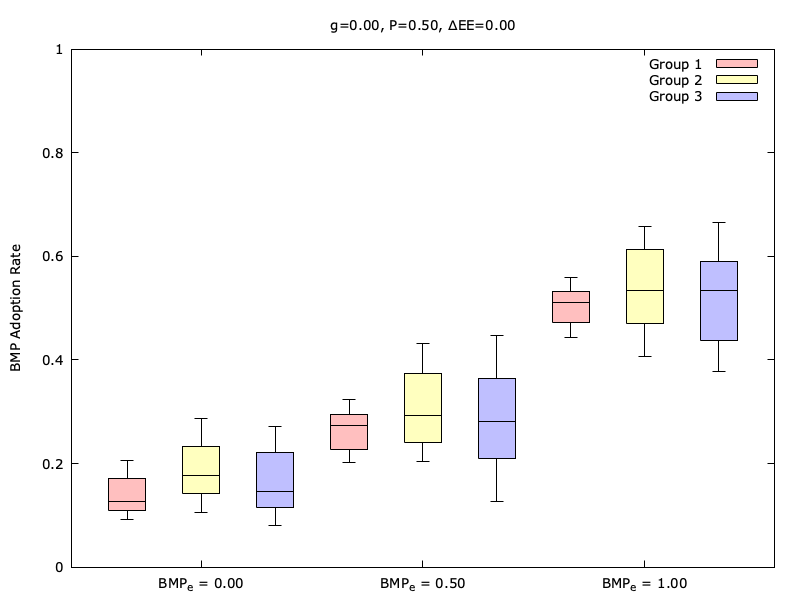
\includegraphics[width=.3\textwidth]{figure/g0P50}}
    \hfill
    \subcaptionbox{$P=0.75$}{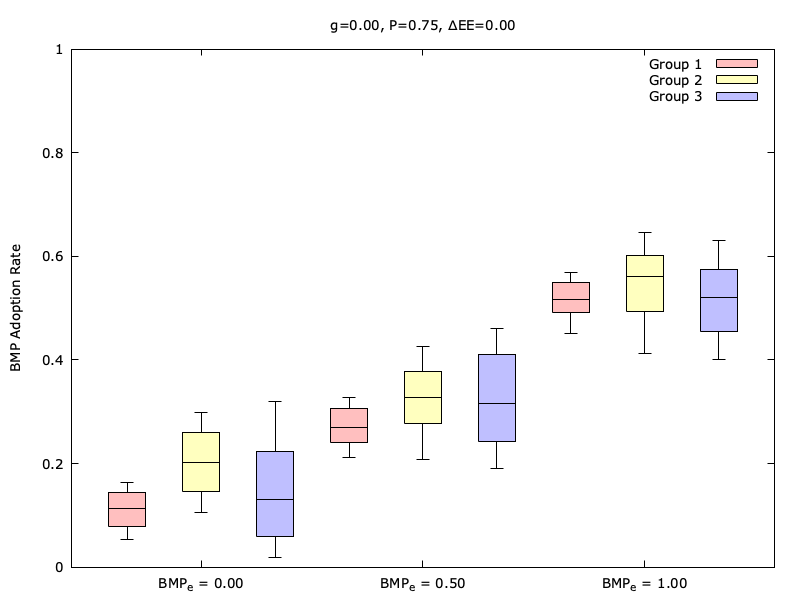
\includegraphics[width=.3\textwidth]{figure/g0P75}}
    \caption{Distribution of mean BMP adoption rate for mixed population
        runs of the agricultural land use model, where $g=0.0$,
        $\Delta EE=0$,
        for (a) $P=0.25$, (b) $P=0.5$, and (c) $P=0.75$}
    \label{fig:farm_res_mix0}
\end{figure}


\section{Discussion}
\label{sec:farm_disc}

Overall, results seem to indicate that this method of introducing
deep reinforcement learning into agent-based modeling does have some
viability for driving agent decision-making;
however,
some components of the experimental testing show how sensitive this
kind of model can be be to its parameterization.

The purpose of the regulatory agent in the experimental model was
to help incentivize specific agent behaviors, but the experimental
parameter being used ($g$) had such a strong impact on the variability
in agent behavior that the results of model runs where $g=0.2$
had such high variance that it is difficult 

Similarly,
in the mixed population runs, the experimental method for introducing
heterogeneity into the population can introduce variance in observed
behaviors, but further testing would be needed to know if it leads
to any of the desired emergent behavioral patterns.
An experimental study specifically targeting an analysis of
the heterogeneity in behaviors seen in real-world populations
would be an ideal next-step.

\chapter{Increasing ABM Integration}
\label{chap:land}

% The last chapter was about the agricultural land-use ABM
% This chapter is going to be about the land-cover transition ABM
% This model also uses deep reinforcement learning in order to train agents
% The goal of this model is to demonstrate the predictive accuracy of the model
% and to prove the viability of the methodology, that being,
% that adding learning to an ABM allows for more meaningful decision-making
% AND that the ABM part allows the learning to capture features that
% might be hard to model otherwise

The previous chapter demonstrated how an agent-based model can be
implemented with machine learning in order to induce a model of
individual behavior.
This chapter will go on to show how this kind of agent-based model
can be integrated with a land cover model in order to predict
land cover change.

\section{Methodology}
\label{sec:land_methods}

The methodology here expands on the methodology presented in 
Chapter~\ref{chap:farm}.
This model is also an agent-based model, but instead of
focusing primarily on training the decision-policy of agents in the model,
the focus is on the land cover change that results as a byproduct of the
behavior of the agents.

\subsection{Modeling Land Cover Change}
\label{subsec:land_methods_cover}

Within the model, land cover is represented as a grid of cells.
Each cell has a land cover category, an NLCD land cover class,
a land use, and an associated land parcel. See Table~\ref{tab:land_cells}.

\begin{table}
\centering
\caption{Land Cell Features}
\label{tab:land_cells}
\begin{tabular}{llll}
\hline
\hline
    Parameter & Values \\
    \hline 
    Land Cover Category & Agricultural, Forested, Urban, Other \\
    NLCD Cover Class &  \\
    Land Usage Type & Managed/In-Use, Adjacent, Unmanaged \\
    \hline
\end{tabular}
\end{table}

Land cover change is modeled as a stochastic byproduct of agent
decision-making.
For example,
an agricultural agent deciding to increase its productivity
with regard to grazing animals may result in clearing forested land cells
and transitioning them to pasture.

These land-cover transitions 

Agent behavior is trained according to internal incentive structures,
the model and was trained on the validation accuracy of transitions
between land cover types in the validation dataset.

\begin{table}
\centering
\caption{Land Cover Categories}
\begin{tabular}{llc}
\hline
\hline
    Cover Category & NLCD Cover Class & Encoding \\
\hline
    Urban & Open Space Urban & 21 \\
    & Low Density Urban & 22 \\
    & Medium Density Urban & 23 \\
    & High Density Urban & 24 \\
    Forested & Deciduous Forest & 41 \\
    & Evergreen Forest & 42 \\
    & Mixed Forest & 43 \\
    Agricultural 
    & Pasture & 81 \\
    & Crops & 82\\
    Barren & Barren & 31 \\
    Grassland/Scrub & Scrub & 52 \\
    & Grassland & 71 \\
    Other & Water & 11 \\
    & Wetlands Woody & 90 \\
    & Wetlands Other & 95 \\
\hline
\end{tabular}
\end{table}

\textbf{Details}

%\subsection{Agent Networks and Connectivity}
%\label{subsec:land_methods_networking}

\section{Experimental Design}
\label{sec:land_exp}

\subsection{The Model}
\label{subsec:land_exp_model}

Real world land cover datasets for years: 2006, 2011, 2016.
Real world land cover transitions between 2006 and 2011 were
used as training and validation data for the land cover model.
Real world land cover transitions between 2011 and 2016 were
used as test data for the land cover model.

The real world transitions mapped from cover $A$ to cover $B$,
which is referred to as $\Delta_{A,B}$.
The modeled transitions for a parameterization $M(...)$ from cover $A$
to cover $\hat{B}$ is referred to as $\Delta_{A,\hat{B}}M(...)$.

\textbf{Explain meaning}

\subsubsection{Agents}
\label{subsubsec:land_exp_agents}

There are four types of agent present in this model:
agricultural agents,
forestry agents,
commercial agents, and
residential agents.

Agricultural agents model the behavior of farmers, herders, and other kinds of 
agricultural land managers within the study area.
They make annual decisions about their farming practices,
including whether they should change production in one of the four modeled 
agricultural industries (beef, dairy, corn, and hay) 
and whether they should implement an agricultural best management practice 
(BMP) to reduce phosphorous runoff on their land.
This agent type is very similar to how it was implemented in the
previous model; although, now, its productivity decisions can change
the land cover of the model.

Forester agents model the behavior of loggers and other kinds of
forested land managers within the study area.
They make annual decisions about their practices
and whether to implement an advised management practice (AMP).

Commercial agents model the behavior of shops, factories, offices, 
and other kinds of commercial land-holders within each study area. 
They make decisions trimonthly about their workforce, 
including their available jobs and the associated salaries
Byproducts of their actions impact the density and sprawl of urban
land cover on the landscape.

Residential agents model the behavior of renters and landowners within 
each study area. 
They make two decisions annually: whether to attempt a job change and whether 
to try to move house. 
Household satisfaction is valued as a combination of financial stability and 
mental satisfaction. 
Each household earns wages provided by a commercial agent --- 
these wages are determined by a stochastic process and can be adjusted by the 
job over time.
The decisions of these agents do not directly impact land cover change
on their associated parcel, but land cover can transition within their
parcel as a result of the decisions of other agents.

Agricultural and forestry agents are connected to and share information with
their $n$-nearest neighbors of the same agent type; these
networks are static throughout each model run.
Commercial and residential agents exist in a bipartite network with
one another.
This network is initialized via a stochastic process and is
updated as agents make decisions.

The learning architecture for agents of each type is
listed in Table~\ref{tab:land_anns}.

\begin{table}
\centering
\caption{Network parameters for the ANNs used by agents in each class
    for the land cover model}
\label{tab:land_anns}
    \begin{tabular}{@{\extracolsep{4pt}}lp{.05\linewidth}>{\centering}p{.05\linewidth}>{\centering}p{.05\linewidth}>{\centering}p{.05\linewidth}>{\centering}p{.05\linewidth}>{\centering}p{.05\linewidth}>{\centering}p{.05\linewidth}cc@{}}
\hline
\hline
\multirow{2}{*}{Parameter} 
    & \multicolumn{2}{c}{Agricultural} & \multicolumn{2}{c}{Forestry} 
    & \multicolumn{2}{c}{Commercial} & \multicolumn{2}{c}{Residential} \\
    \cline{2-3}\cline{4-5}\cline{6-7}\cline{8-9}
 & $\mu$ & $Q$ & $\mu$ & $Q$ & $\mu$ & $Q$ & $\mu$ & $Q$  \\
\hline
Input Nodes  & 15 & 32 & 10 & 15 & 4 & 10 & 5 & 9 \\
Inner Layers  & 4 & 3 & 4 & 3 & 2 & 2 & 2 & 2 \\
Inner Nodes  & 10 & 16 & 7 & 7 & 5 & 5 & 4 & 5 \\
Output Nodes  & 17 & 1 & 5 & 1 & 6 & 1 & 4 & 1 \\
\hline
\end{tabular}
\end{table}

\subsubsection{Execution Overview}
\label{subsubsec:land_exp_exe}

\textbf{Add Textual description of model execution and the timing of
model subsystems. Agents make decisions, then act and interact, then learn.}

\begin{figure}
\centering
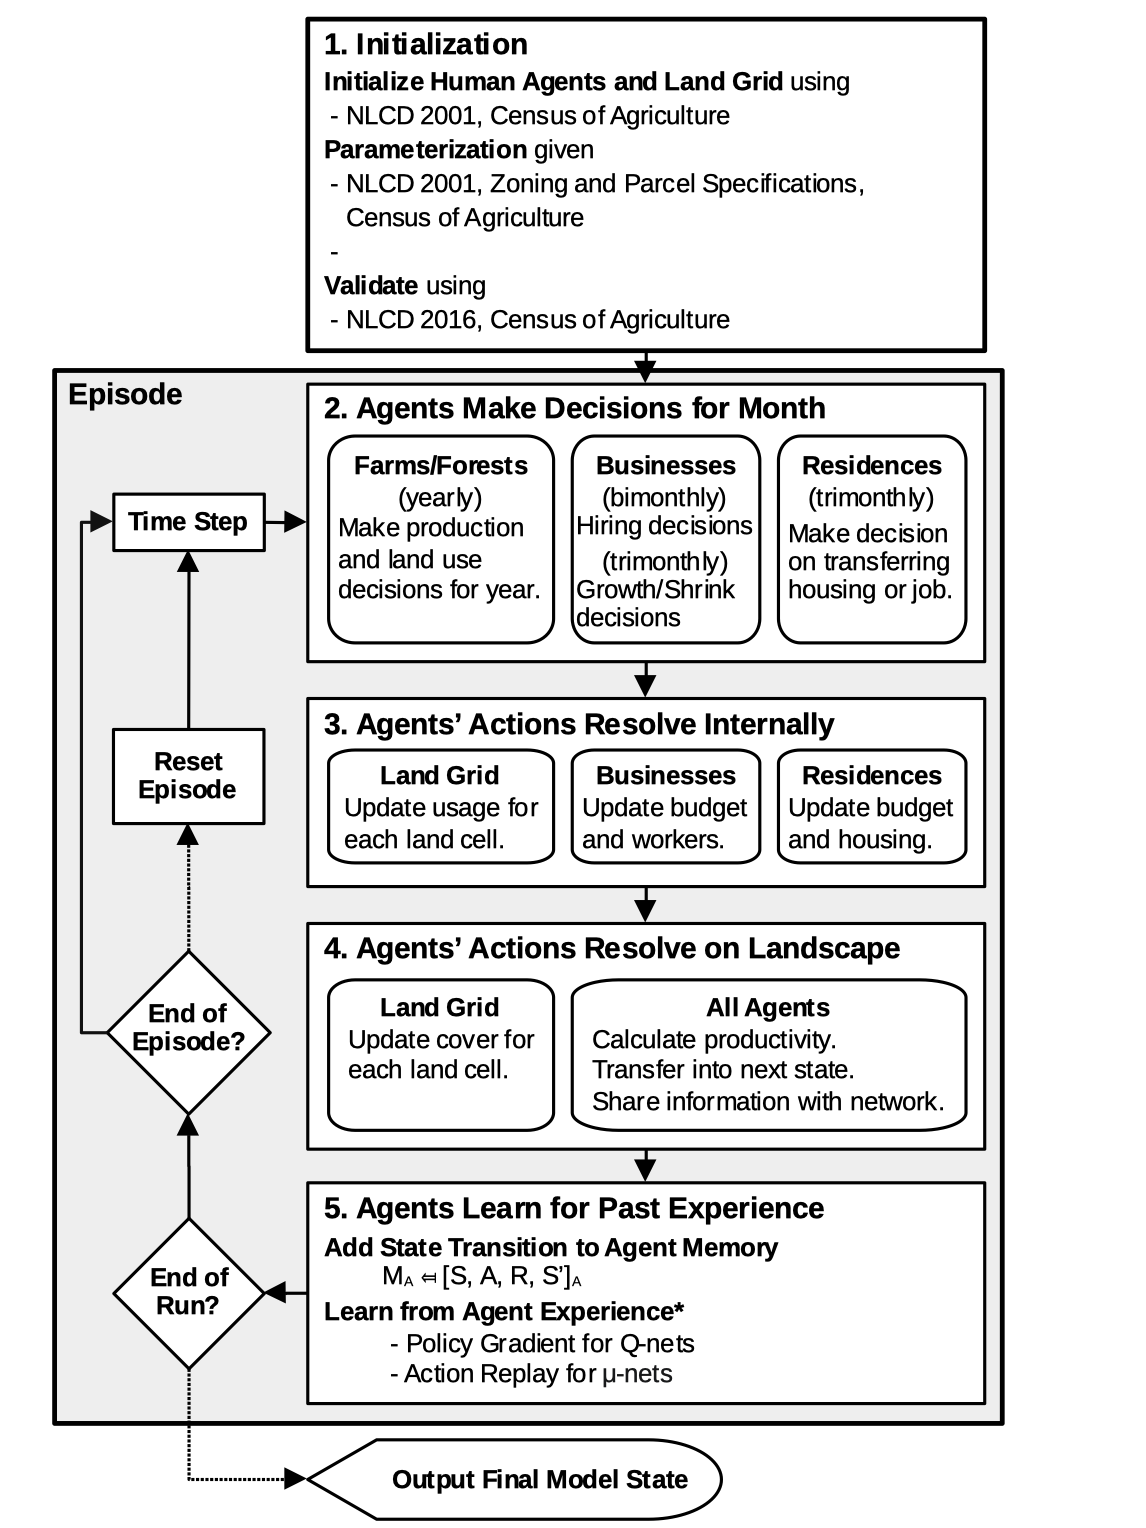
\includegraphics[width=0.7\textwidth]{figure/flowchart1.png}
\caption{Flowchart demonstrating the overall execution of the agent-based model
    and its coupling with the machine learning process}
\end{figure}

\subsection{Hyperparameter Selection}
\label{subsec:land_exp_hyper}

A summary of model hyperparameters is listed in Table~\ref{tab:land_hyper}.

\subsection{Experimental Setup}
\label{subsec:land_exp_setup}

Parameters were varied for experimental scenarios.

\textbf{Explain why this is more of a hyperparameter analysis. Because
we want to explore how agent interactivity and agent decision-making can
have secondary effects.}

\textbf{Include other parameters, or simple version?}

\begin{table}
\caption{Experimental parameters for the land cover transition model}
\centering
\begin{tabular}{ll}
\hline
\hline
    Variable & Values \\
    \hline
    Batch Size ($B$) & 8, 16, 32, 64 \\
    Discount Factor ($\gamma$) & 0.5, 0.9, 0.99 \\
%    Population Mixing ($P$) & 0.0, 0.25, 0.5, 0.75 \\
    Recall Accuracy ($F'$) & 0.0, 0.25, 0.5, 0.75 \\
    \hline
\end{tabular}
\end{table}

% As a second measure of model performance, a convolutional neural network (CNN)
% was trained on the same data as the agent-based model.
% The CNN was trained to predict the land cover of a cell at time $t_e$
% based on the land cover of the cell and it's surrounding neighborhood
% at time $t_s$.
% 
%     \^{C}=CNN(A)
% 
%     $\hat{C}=ConvNet(A)$
% 
% Parameters for the comparative CNN model.
% 
% \begin{table}
% \centering
%     \caption{Network architecture of comparative CNN}
%     \label{tab:land_cnn}
%     \begin{tabular}{lcccc}
%         \hline
%         \hline
%         Layer & Size & Stride & Kernel & Activation \\
%         \hline
%         Input & $5\times 5$ & 1 & --- & --- \\
%         Convolutional & $5\times 5$ & 1 & 6 & ReLU \\
%         Pooling & $2\times 2$ & 2 & --- & --- \\
%         Convolutional & $5\times 5$ & 1 & 16 & ReLU \\
%         Pooling & $2\times 2$ & 2 & --- & --- \\
%         Fully Connected & 120 & --- & --- & ReLU \\
%         Fully Connected & 84 & --- & --- & ReLU \\
%         Output & 17 & --- & --- & Softmax \\
%         \hline
%     \end{tabular}
% \end{table}

\subsection{Known Limitations}
\label{sec:land_lim}

Some types of land-cover transition either do not exist in the training
data or are not well-represented.
These types of transitions are rare within the study area,

\textbf{move and elaborate}

% For the purposes of analyzing the results of this model,
% where these types of transitions occur,
% they are treated as neither a successful nor an unsuccessful measure
% of model performance.
% Instead, they are treated as a separate neutral measure.
% 
% This limitation of the model is discussed in greater detail
% in Section~\ref{sec:land_disc}.
% 
% 
% For many of these missing transitions,
% there is a lack of any substantive literature supporting a predictive model 
% that is generalizable enough to meaningfully incorporate into the ABM.


\section{Results}
\label{sec:land_results}

\subsection{Model Performance}
\label{subsec:land_results_performance}

Model performance under each experimental parameterization was
evaluated by comparing the land cover in model year 2016 to
the recorded/observed land cover for the study area for real year 2016.

The Nash-Sutcliffe efficiency index (NSE) was used to evaluate
the goodness-of-fit of the model under each experimental parameterization.
The NSE is a measure of the relative magnitude of the residual variance
of modeled data compared to the residual variance of the observed data.
The value of the index ranges from $-\inf$ to $1$,
where a score of 1 indicates a perfect fit,
a score of 0 indicates that the model is no better than the mean of the
observed data,
and a score less than 0 indicates that the mean of the observed data
is a better predictor than the model.

This index was calculated in relation to three forms of model performance.
The first is the ability of the model to appropriately predict
the proportional coverage of each land cover type in the target year,
$\text{NSE}_\text{plc}$.
The second is the ability of the model to appropriately predict
the categorical transitions of land cover types from the start year to
the target year,
$\text{NSE}_\text{cat}$.
The third is the ability of the model to appropriately predict
the absolute transitions of land cover types from the start year to
the target year,
$\text{NSE}_\text{abs}$.
These indices are detailed below.

A majority of land cells in the study area do not transition land cover
between the start year and target year ($92.6\%, n=69124$),
which would heavily bias any analysis of model performance.
Therefore, the NSE was calculated only for those cells that transitioned
land cover.

The NSE measure of proportional coverage ($\text{NSE}_\text{plc}$),
shown in Equation~\ref{eq:nse_plc},
where $P_b$ represents the observed proportional coverage of land cover
type $b$ in the target year,
$\hat{P_b}$ represents the simulated proportional coverage of land cover
type $b$ in the target year,
and $\bar{P_b}$ represents the mean observed proportional coverage of
land cover type $b$ in the target year.

\begin{equation}
    \label{eq:nse_plc}
    \text{NSE}_{\text{plc}} 
    = \frac{\sum_b\left(P_b - \hat{P_b}\right)^2}
        {\sum_b\left(P_b-\bar{P_b}\right)^2}
\end{equation}

The NSE measure of categorical land cover transitions ($\text{NSE}_\text{cat}$),
shown in Equation~\ref{eq:nse_cat},
where $\Delta_{A,B}$ represents the number of observed transitions
from land cover category $A$ in the starting year to land cover
category $B$ in the target year,
where $\widehat{\Delta_{A,B}}$ represents the number of simulated transitions
from $A$ to $B$,
and where $\overline{\Delta_{A,B}}$ represents the mean observed number of
transitions from $A$ to $B$. \textbf{Not sure I'm saying this correctly.}

\begin{equation}
    \label{eq:nse_cat}
    \text{NSE}_{\text{cat}}
    = \frac{\sum_{A,B}\left(\Delta_{A,B}-\widehat{\Delta_{A,B}}\right)^2}
        {\sum_{A,B}\left(\Delta_{A,B}-\overline{\Delta_{A,B}}\right)^2},
    A \ne B
\end{equation}

The NSE measure for absolute land cover transition ($\text{NSE}_\text{act}$),
shown in Equation~\ref{eq:nse_act},
is very similar to the calculation of $\text{NSE}_\text{cat}$,
except that it is calculated for the absolute land cover class of each
land cell and not just its categorical class.
\textbf{NLCD Cover Class vs Coverage Category, f.x. for-deciduous vs forested}

\begin{equation}
    \label{eq:nse_act}
    \text{NSE}_{\text{abs}} 
    =
    \frac{\sum_{a,b}\left(\Delta_{a,b} - \widehat{\Delta_{a,b}}\right)^2}
        {\sum_{a,b}\left(\Delta_{a,b} - \overline{\Delta_{a,b}}\right)^2}
    ,
    a\ne b
\end{equation}

The maximum NSE values seen during testing runs were 
$\text{NSE}_\text{plc}=0.84$,
$\text{NSE}_\text{cat}=0.76$, and
$\text{NSE}_\text{act}=0.64$.

The sensitivity of NSE to each model parameterization across model
runs was evaluated by calculating the mean and variance of the NSE indices
under each parameterization. Figure~\ref{fig:land_nse}

\begin{figure}
    \centering
    \subcaptionbox{$\text{NSE}_\text{plc}$}{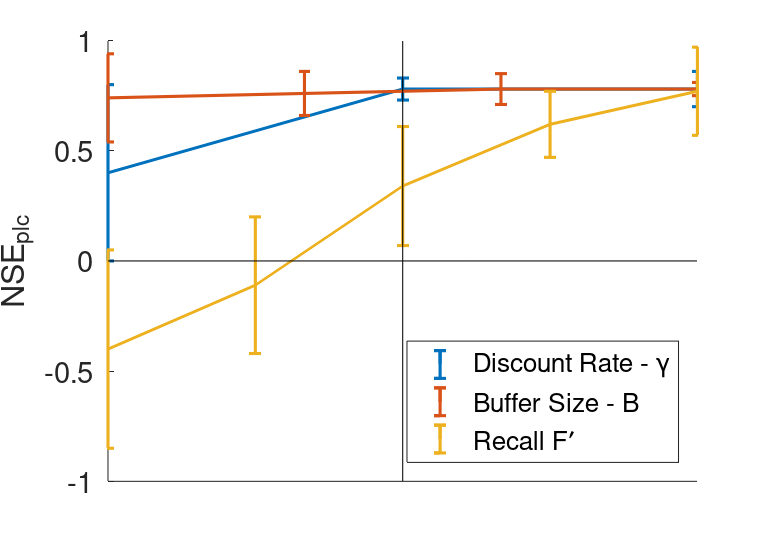
\includegraphics[width=0.3\textwidth]{figure/nscplc}}
    \hfill
    \subcaptionbox{$\text{NSE}_\text{cat}$}{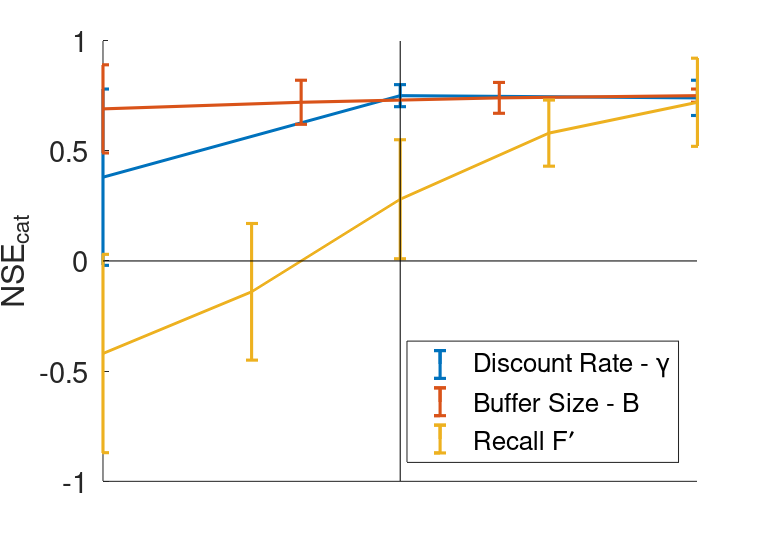
\includegraphics[width=0.3\textwidth]{figure/nsccat}}
    \hfill
    \subcaptionbox{$\text{NSE}_\text{act}$}{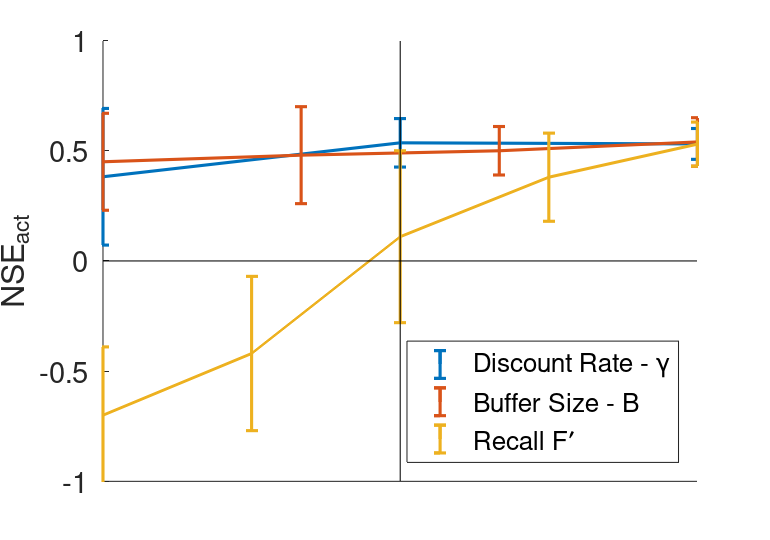
\includegraphics[width=0.3\textwidth]{figure/nscact}}
    \caption{NSE index sensity for each index showing the variance in
    model classification accuracy by each metric under different model
    parameterizations.}
    \label{fig:land_nse}
\end{figure}

\section{Discussion}
\label{sec:land_disc}

\textbf{Explain why it matters.}



\newpage

\setstretch{1.0}
\nocite{*}
\bibliography{bibfile}
\bibliographystyle{unsrt}

\addtocontents{toc}{\protect\setcounter{tocdepth}{1}}
\appendix
\chapter{Farm Model ODD+D Document}
\label{app:farm}

text

\chapter{Land-Cover Model Design Overview}
\label{app:land}

This appendix contains an overview of the design of the land-cover transition
model described in Chapter~\ref{chap:land}.
It generally adheres to the technical principles of the ODD+D format,
as shown in Appendix~\ref{app:farm},
but is focused on where the specification provides details that do not appear
in the main text of this thesis.

\section{Overview}
\subsection{Purpose}
The purpose of this model is to explore potential changes to land cover as a result of human behavior as it develops in response to projected climatological, economic, and social scenarios within study areas of the Lake Champlain Basin of Vermont.
Four types of human agents are present in this model; these agents represent some of the various types of people who make decisions that can change land cover on the landscape. Agents received input from their environment, including inter-agent communication and stochastic environmental factors (f.x. simulated extreme weather events). Agents made decisions as frequently as once per model month, and the decision policy guiding their decision-making was trained using deep reinforcement machine learning.

\subsection{Entities, State Variables, and Scales}

\subsubsection{Study Area}
The study area being used as the basis of this model is a subsection 
of the Lake Champlain Basin of Vermont. 
Each parcel within the study area is treated as an agent within the model.
A map of the study area and its initial land-cover is
shown in Figure~\ref{fig:land_cells}.

\subsubsection{Agents}

There are four types of human agents present in this model --- agricultural,
commercial, residential, and forester. 
These agents represent various types of landowners/managers within each 
study area who are able to make decisions that can affect land-use 
and land-cover. 
They make these decisions based on both their material state 
and their perceived mental and financial state. 
Agent behavior is trained using deep reinforcement machine learning, 
which provides each agent with a decision-policy that guides their 
decision-making during test model runs.

The state variables that are present in every human agent in the model are outlined in Table~\ref{tab:land_state_share}

\begin{longtable}{lcp{0.5\linewidth}l}
\caption{Table of all properties that are shared amongst all human
agents in the land-cover transition model.}
\label{tab:land_state_share} \\
\hline\hline
Name && Description & Data type \\
\hline\endfirsthead
\caption[]{(continued...)}\\
\hline\hline
Name && Description & Data type \\
\hline\endhead
\hline\endfoot
Agent ID && Unique identifier for this agent & \tt{uint} \\
Parcel ID && Identifier of underlying land cell parcel & \tt{uint} \\
Agent Status 
&& Class-dependent internal status & \tt{enum} \\
\multicolumn{4}{l}{Neural Networks} \\
\multicolumn{1}{r}{Actor Network} & $\Theta_\mu$ & Network Weights & \tt{float[][]} \\
\multicolumn{1}{r}{Critic Network} & $\Theta_Q$ & Network Weights & \tt{float[][]} \\
\multicolumn{1}{r}{Target Actor} & $\Theta_{\mu'}$ & Network Weights & \tt{float[][]} \\
\multicolumn{1}{r}{Target Critic} & $\Theta_{Q'}$ & Network Weights & \tt{float[][]} \\
\end{longtable}

\subsubsection*{Agricultural Agents}
Agricultural agents model the behavior of farmers, herders, and other kinds of agricultural land managers within each study area. They make annual decisions about their farming practices, including whether they should change production in one of the four modeled agricultural industries (beef, dairy, corn, and hay) and whether they should implement an agricultural best management practice (BMP) to reduce phosphorous runoff on their land.
The additional state variables that are found in every agricultural agent in the model are outlined in Table~\ref{tab:land_farm_state}.

\begin{longtable}{lcp{.4\linewidth}l}
\caption{Table of all state properties of agricultural agents and their
associated data type for agricultural agents in the land-cover transition model.}
\label{tab:land_farm_state} \\
\hline \hline
Name && Description & Data Type \\
\hline
\endfirsthead
\caption[]{(continued...)}\\
\hline\hline
Name && Description & Data Type \\
\hline\endhead
\hline\endfoot
\multicolumn{4}{l}{Land Parcel Data (sq~km)} \\
\multicolumn{1}{r}{Crop Land Area} & $A_c$ & Land devoted to growing crops & \tt{float} \\
\multicolumn{1}{r}{Pasture Land Area} & $A_p$ & Land devoted to grazing animals & \tt{float} \\
\multicolumn{1}{r}{Total Land Area} & $A_{tot}$ & Total land in parcel & \tt{float} \\
\multicolumn{4}{l}{Land Cover (Cell Count)} \\
& $c_{c,m}$ & Cropland/In-use & \tt{uint} \\
& $c_{c,a}$ & Cropland/Adjacent & \tt{uint} \\
& $c_{p,m}$ & Pasture/In-use & \tt{uint} \\
& $c_{p,a}$ & Pasture/Adjacent & \tt{uint} \\
& $c_{a,u}$ & Agricultural/Unmaintained & \tt{uint} \\
& $c_{o,a}$ & Other/Adjacent Cell Count & \tt{uint} \\
Productivity \\
\multicolumn{1}{r}{Corn} & $p_c$ & Corn production factor & \tt{float} \\
\multicolumn{1}{r}{Hay} & $p_h$ & Hay production factor & \tt{float} \\
\multicolumn{1}{r}{Beef} & $p_b$ & Beef production factor & \tt{float} \\
\multicolumn{1}{r}{Dairy} & $p_d$ & Dairy production factor & \tt{float} \\
\multicolumn{1}{r}{Phosphorous} & $p_{p,x}$ & Phosphorus production factors & \tt{float[3]} \\
Cows Owned &&& \tt{uint} \\
\multicolumn{4}{l}{Financial History (5-year)} \\
\multicolumn{1}{r}{Realized Net} && Net yearly production & \tt{float[5]} \\
\multicolumn{1}{r}{Expected Net} && Expected yearly production& \tt{float[5]} \\
Extreme Event History &&& \tt{bool[5]}\\
BMP Usage History && Did farm use BMP in last 5 years & \tt{bool[5]} \\
Neighbors && References to neighboring agents & \tt{uint[5]} \\
\end{longtable}

\subsubsection*{Forestry Agents}

Forestry agents model the behavior of loggers and other kinds of
forested land managers within the study area.
They make annual decisions about their practices
and whether to implement an advised management practice (AMP)
on their land.
The forestry agents are implemented very similarly to the
agricultural agents, but the land-cover of interest has been changed
to forested land, and the production function has been replaced with
a generalized forested productivity function.
The additional state factors used by the forestry agents in their decision-making
are listed in Table~\ref{tab:land_state_for}.

\begin{longtable}{lcp{.4\linewidth}l}
\caption{Table of state properties of forestry agents and their
associated data types in the land-cover transition model.}
\label{tab:land_state_for} \\
\hline \hline
Name & & Description & Data Type \\ \hline
\endfirsthead
\hline \hline
Name & & Description & Data Type \\ \hline
\endhead
\hline\endfoot
\multicolumn{4}{l}{Land Parcel Data (sq~km)} \\
\multicolumn{1}{r}{Forested Land Area} & $A_p$ & Total forested land in parcel & \tt{float} \\
\multicolumn{1}{r}{Total Land Area} & $A_{tot}$ & Total land in parcel & \tt{float} \\
\multicolumn{4}{l}{Land Cover (Cell Count)} \\
& $c_{f,m}$ & Forested/In-use & \tt{uint} \\
& $c_{f,a}$ & Forested/Adjacent & \tt{uint} \\
& $c_{f,u}$ & Forested/Unmaintained & \tt{uint} \\
& $c_{o,a}$ & Other/Adjacent Cell Count & \tt{uint} \\
\multicolumn{4}{l}{Productivity} \\
\multicolumn{1}{r}{General} & $p_f$ 
    & Relative production factor & \tt{float} \\
\multicolumn{1}{r}{Phosphorous} & $p_p$
    & Relative production factor & \tt{float} \\
\multicolumn{4}{l}{Financial History (5-year)} \\
\multicolumn{1}{r}{Realized Net} && Net yearly production & \tt{float[5]} \\
\multicolumn{1}{r}{Expected Net} && Expected yearly production & \tt{float[5]} \\
Extreme Event History &&& \tt{bool[5]}\\
AMP Usage History && Did agent use AMP in last 5 years & \tt{bool[5]}\\
Neighbors & & References to neighboring agents & \tt{uint[5]} \\
\end{longtable}

\subsubsection*{Commercial Agents}

Commercial agents model the behavior of shops, factories, offices, 
and other kinds of commercial land-holders within the study area. 
They make decisions bi/trimonthly about their workforce, 
including their available jobs and the associated salaries.
Byproducts of their actions impact the density and sprawl of urban
land cover on the landscape.
The additional state factors that it uses in decision-making are listed
in Table~\ref{tab:land_state_com}.

\begin{longtable}{lcp{.45\linewidth}l}
\caption{Table of state properties of commercial agents and their
associated data types in the land-cover transition model.}
\label{tab:land_state_com} \\
\hline \hline
Name & & Description & Data Type \\ \hline
\endfirsthead
\hline \hline
Name & & Description & Data Type \\ \hline
\endhead
\hline\endfoot
Days Operational && Number of days operating & \tt{uint}\\
Employee Count && Current number of employed agents & \tt{uint}\\
Employee Capacity && Maximum number of employed agents & \tt{uint}\\
Employee IDs && IDs of employed agents & \tt{uint*}\\
Employee Salaries && Salaries of employed agents & \tt{float*}\\
Total Pay && Total salaried paid to all employees & \tt{float} \\
Budget && Total monthly budget & \tt{float} \\
\end{longtable}

\subsubsection*{Residential Agents}

Residential agents model the behavior of renters and landowners within 
the study area. 
They make two decisions annually: whether to attempt a job change 
and whether to try to move houses. 
Household satisfaction, and their reward value~$R_r$,
is valued as a combination of financial stability 
and mental satisfaction. 
Each household earns wages provided by a commercial agent --- 
these wages are determined by a stochastic process and can be adjusted by 
the job over time.
The decisions of these agents do not directly impact land cover change
on their associated parcel, but land cover can transition within their
parcel as a result of the decisions of other agents.

\begin{longtable}{lcp{.5\linewidth}l}
\caption{Table of state properties of residential agents and their
associated data types in the land-cover transition model.}
\label{tab:land_state_res} \\
\hline \hline
Name & & Description & Data Type \\ \hline
\endfirsthead
\hline \hline
Name & & Description & Data Type \\ \hline
\endhead
\hline\endfoot
Employer ID && ID of current employer & \tt{uint} \\
Housing Costs && Total monthly cost of living & \tt{float} \\
Salary && Total monthly income from employer & \tt{float} \\
Monthly Budget && Net income over past 1 month & \tt{float} \\
Yearly Budget && Net income over past 12 months & \tt{float[12]} \\
Time in State && Number of time steps with current `mood' & \tt{uint} \\
Failed Action Count && Number of consecutive failed actions & \tt{uint} \\
\end{longtable}

\subsection{Process Overview and Scheduling}

Each time-step within the model is representative of one modeled month.
Each model year (12 time-steps), the number of extreme weather events for the year are
generated and the agricultural and forestry agents act.

The commercial agent has two primary decision-vectors,
the decision to increase or decrease overall productivity is resolved trimonthly (3 time-steps),
while the decision to hire/fire staff is resolved bimonthly (2 time-steps).
At the end of each model year (12 time-steps), the commercial agent will increase the
salary of all employed residential agents by 10\%.

A commercial agent which loses its last employee,
by firing or quitting, will enter the ``bankrupt'' state at the end of
the occurent time-step, and will not be replaced with a ``new'' commercial agent until
3 time-steps have passed.
This new agent has a period of 3--6 time-steps to acquire its first employee before it
can bankrupt again.

The residential agent acts monthly (1 time-step); however, its actions are dependant
on the behavior of other agents in the model --- f.x. a residential agent cannot move
into an occupied house regardless of its price.
If a residential agent intends to leaves its job, house, or the entire system,
this action cannot be blocked, it is only additive actions which face this restriction.

A new residential agent may only enter the system if there is an available residential
parcel with an occupation status of ``vacant'' or ``for-sale''
and the total number of residential agents within the system does not match nor exceed
the current residential capacity.
This new residential agent will be added to the system at the start of the following
time-step.

\section{Initialization}

\subsection{Agent Connections}

Agricultural and forestry agents are all connected to their
5-nearest agents of the same type.
Since these agents do not move on the landscape, these networks are
constant throughout each model run.

Commercial and residential agents exist within a bipartite network.
During model initialization, each commercial agent starts with an
employment capacity of 10.
At model start, 90\% of residential agents are assigned jobs
selected with uniform likelihood from that available commercial capacity.
The initial employment capacity within the selected study area ensures that
there will always be more initial capacity than 90\% of the initial residential capacity.
These networks are dynamic and change as agents make decisions throughout each model run.

\subsection{Initial Agent State}

Many of these values are selected from triangular distributions
which was parameterized according to the calibration of the
underlying economic model.
Triangular distributions, as described in Section~\ref{sec:farmer_init},
are used for the initialization of many parameters.
Neural networks had weights initialized according to the He~initialization
algorithm.~\cite{he2004initialization}.

\begin{longtable}{lcll}
\hline\hline
Value & & Initialization & Type \\
\hline
\endhead
\hline\endfoot
Agent ID & & Assigned sequentially from 0 & \tt{uint} \\
Parcel ID & & Read from Input Data & \tt{uint} \\
Actor-Network Weights & $\Theta_\mu$ & He() & \tt{float[][]} \\
Critic-Network Weights & $\Theta_Q$ & He() & \tt{float[][]} \\
Target-Actor Weights & $\Theta_{\mu'}$ 
    & Copied from $\Theta_\mu$ & \tt{float[][]} \\
Target-Critic Weights & $\Theta_{Q'}$ 
    & Copied from $\Theta_Q$ & \tt{float[][]} \\
\end{longtable}

\subsubsection*{Agricultural Agents}
\label{sec:land_farmer_init}
Many of the initial values used by the agricultural agents are initialized
from the input data.
The variables which are set during initialization are listed in
Table~\ref{tab:land_farmer_init}.

\begin{longtable}{lcll}
    \caption{Table listing initialization of parameters of
    the agricultural agents in the land-cover transition model}
    \label{tab:land_farmer_init}
    \\
    \hline\hline
    Value & & Initialization & Type \\
    \hline
    \endfirsthead
    \caption[]{(continued ...)}\\ \hline\hline
    Value & & Initialization & Type\\ \hline
    \endhead
    \hline
    \endfoot
    Parcel Data & $A_x$ & 
    Read from input file & \tt{float} \\
    Corn Production (USD) & $p_c$ 
        & $\Tri_2(3.362551, 4259232)$ & \tt{float} \\
    Corn Production (P) & $p_{p,c}$ 
        & $\Tri_2(\SI{2.02e-4}{}, \SI{6.17e-4}{})$ & \tt{float} \\
    Hay Production (USD) & $p_h$ 
        & $\Tri_2(0.358672, 0.470757)$ & \tt{float} \\
    Hay Production (P) & $p_{p,h}$
        & $\Tri_2(\SI{3.37e-5}{}, \SI{1.12e-4}{})$ & \tt{float} \\
    Beef Production (USD) & $p_b$ & $\Tri_2(900.0, 1200.0)$ & \tt{float} \\
    Dairy Production (USD) & $p_d$ & $\Tri_2(210.0, 250.0)$ & \tt{float} \\
    Cow Production (P) & $p_{p,[bd]}$ 
        & $\Tri_2(\SI{3.366e-4}{}, \SI{7.853e-4}{})$ & \tt{float} \\
    Cows Owned & $C$ & $\Tri_2(3600, 7800)$ & \tt{uint} \\
\end{longtable}

\subsubsection*{Residential and Commercial Agents}

Initial agent salaries are selected from the weighted categorical distribution described in
Table~\ref{tab:sals} on the range $\left(250, 1000\right)$.
The initial rent/mortgage price for each urban land parcel is selected from a uniform distribution
on the range $\left(400, 1100\right)$.

\begin{longtable}{ll}
\caption{Table listing distribution of initial agent salaries and the weight on their probability.}\label{tab:sals}\\
\hline\hline
Weight & Initial Salary \\
\hline\endfirsthead
\hline\hline
Weight & Initial Salary \\
\hline\endhead
\hline\endfoot
    10 & 250 \\
    20 & 300 \\
    30 & 350 \\
    50 & 400 \\
    70 & 450 \\
    85 & 500 \\
    90 & 550 \\
    85 & 600 \\
    70 & 650 \\
    60 & 700 \\
    50 & 750 \\
    50 & 800 \\
    50 & 850 \\
    50 & 900 \\
    30 & 950 \\
    20 & 1000 \\
\end{longtable}
\chapter{Result Listings}
\label{app:results}

This appendix contains listings of model results which would be difficult to display alongside
the main text.

\begin{longtable}{ccccc}
    \caption{Mean BMP~adoption rate for uniform-population runs of the agricultural model for 
    the parameterizations with results plotted in Figure~\ref{fig:farm_res_g00}, Figure~\ref{fig:farm_res_g05}, and
    Figure~\ref{fig:farm_res_g20}.} \\
    \label{tab:full_res_uniform} \\
    \hline
    \hline
    $g$ & $F$ & $BMP_e$ & $\Delta EE$ & Adoption Rate \\
    \hline
    \endfirsthead
    \caption[]{(continued...)}\\
    \hline
    \hline
    $g$ & $F$ & $BMP_e$ & $\Delta EE$ & Adoption Rate \\
    \hline
    \endhead
    \hline
    \endfoot
    \hline
    \endlastfoot
    % g = 0
    % F = 0
    % BMP_e = 0.0
    0.0 & 0.0 & 0.0 & -0.2  & $0.053$ \\
    0.0 & 0.0 & 0.0 &  0.0  & $0.058$ \\
    0.0 & 0.0 & 0.0 &  0.2  & $0.040$ \\ \hline
    % BMP_e = 0.5
    0.0 & 0.0 & 0.5 & -0.2  & $0.150$ \\
    0.0 & 0.0 & 0.5 &  0.0  & $0.252$ \\
    0.0 & 0.0 & 0.5 &  0.2  & $0.461$ \\ \hline
    % BMP_e = 1.0
    0.0 & 0.0 & 1.0 & -0.2  & $0.349$ \\
    0.0 & 0.0 & 1.0 &  0.0  & $0.505$ \\
    0.0 & 0.0 & 1.0 &  0.2  & $0.759$ \\ \hline
    % F = 0.5
    % BMP_e = 0.0
    0.0 & 0.5 & 0.0 & -0.2  & $0.173$ \\
    0.0 & 0.5 & 0.0 &  0.0  & $0.231$ \\
    0.0 & 0.5 & 0.0 &  0.2  & $0.452$ \\ \hline
    % BMP_e = 0.5
    0.0 & 0.5 & 0.5 & -0.2  & $0.202$ \\
    0.0 & 0.5 & 0.5 &  0.0  & $0.300$ \\
    0.0 & 0.5 & 0.5 &  0.2  & $0.450$ \\ \hline
    % BMP_e = 1.0
    0.0 & 0.5 & 1.0 & -0.2  & $0.399$ \\
    0.0 & 0.5 & 1.0 &  0.0  & $0.488$ \\
    0.0 & 0.5 & 1.0 &  0.2  & $0.589$ \\ \hline
    % F = 1.0
    % BMP_e = 0.0
    0.0 & 1.0 & 0.0 & -0.2  & $0.310$ \\
    0.0 & 1.0 & 0.0 &  0.0  & $0.333$ \\
    0.0 & 1.0 & 0.0 &  0.2  & $0.427$ \\ \hline
    % BMP_e = 0.5
    0.0 & 1.0 & 0.5 & -0.2  & $0.339$ \\
    0.0 & 1.0 & 0.5 &  0.0  & $0.349$ \\
    0.0 & 1.0 & 0.5 &  0.2  & $0.450$ \\ \hline
    % BMP_e = 1.0
    0.0 & 1.0 & 1.0 & -0.2  & $0.411$ \\
    0.0 & 1.0 & 1.0 &  0.0  & $0.491$ \\
    0.0 & 1.0 & 1.0 &  0.2  & $0.529$ \\ \hline
    % g = 0.05
    % F = 0
    % BMP_e = 0.0
    0.05 & 0.0 & 0.0 & -0.2  & $0.106$ \\
    0.05 & 0.0 & 0.0 &  0.0  & $0.124$ \\
    0.05 & 0.0 & 0.0 &  0.2  & $0.121$ \\ \hline
    % BMP_e = 0.5
    0.05 & 0.0 & 0.5 & -0.2  & $0.364$ \\
    0.05 & 0.0 & 0.5 &  0.0  & $0.418$ \\
    0.05 & 0.0 & 0.5 &  0.2  & $0.478$ \\ \hline
    % BMP_e = 1.0
    0.05 & 0.0 & 1.0 & -0.2  & $0.733$ \\
    0.05 & 0.0 & 1.0 &  0.0  & $0.793$ \\
    0.05 & 0.0 & 1.0 &  0.2  & $0.847$ \\ \hline
    % F = 0.5
    % BMP_e = 0.0
    0.05 & 0.5 & 0.0 & -0.2  & $0.092$ \\
    0.05 & 0.5 & 0.0 &  0.0  & $0.088$ \\
    0.05 & 0.5 & 0.0 &  0.2  & $0.094$ \\ \hline
    % BMP_e = 0.5
    0.05 & 0.5 & 0.5 & -0.2  & $0.219$ \\
    0.05 & 0.5 & 0.5 &  0.0  & $0.265$ \\
    0.05 & 0.5 & 0.5 &  0.2  & $0.332$ \\ \hline
    % BMP_e = 1.0
    0.05 & 0.5 & 1.0 & -0.2  & $0.378$ \\
    0.05 & 0.5 & 1.0 &  0.0  & $0.463$ \\
    0.05 & 0.5 & 1.0 &  0.2  & $0.566$ \\ \hline
%    % F = 1.0
%    % BMP_e = 0.0
%    0.05 & 1.0 & 0.0 & -0.2  & $0.$ \\
%    0.05 & 1.0 & 0.0 &  0.0  & $0.$ \\
%    0.05 & 1.0 & 0.0 &  0.2  & $0.$ \\ \hline
%    % BMP_e = 0.5
%    0.05 & 1.0 & 0.5 & -0.2  & $0.$ \\
%    0.05 & 1.0 & 0.5 &  0.0  & $0.$ \\
%    0.05 & 1.0 & 0.5 &  0.2  & $0.$ \\ \hline
%    % BMP_e = 1.0
%    0.05 & 1.0 & 1.0 & -0.2  & $0.$ \\
%    0.05 & 1.0 & 1.0 &  0.0  & $0.$ \\
%    0.05 & 1.0 & 1.0 &  0.2  & $0.$ \\ \hline
    % g = 0.2
    % F = 0
    % BMP_e = 0.0
    0.2 & 0.0 & 0.0 & -0.2  & $0.304$ \\
    0.2 & 0.0 & 0.0 &  0.0  & $0.276$ \\
    0.2 & 0.0 & 0.0 &  0.2  & $0.361$ \\ \hline
    % BMP_e = 0.5
    0.2 & 0.0 & 0.5 & -0.2  & $0.396$ \\
    0.2 & 0.0 & 0.5 &  0.0  & $0.473$ \\
    0.2 & 0.0 & 0.5 &  0.2  & $0.548$ \\ \hline
    % BMP_e = 1.0
    0.2 & 0.0 & 1.0 & -0.2  & $0.667$ \\
    0.2 & 0.0 & 1.0 &  0.0  & $0.695$ \\
    0.2 & 0.0 & 1.0 &  0.2  & $0.733$ \\ \hline
    % F = 0.5
    % BMP_e = 0.0
    0.2 & 0.5 & 0.0 & -0.2  & $0.333$ \\
    0.2 & 0.5 & 0.0 &  0.0  & $0.356$ \\
    0.2 & 0.5 & 0.0 &  0.2  & $0.454$ \\ \hline
    % BMP_e = 0.5
    0.2 & 0.5 & 0.5 & -0.2  & $0.396$ \\
    0.2 & 0.5 & 0.5 &  0.0  & $0.467$ \\
    0.2 & 0.5 & 0.5 &  0.2  & $0.574$ \\ \hline
    % BMP_e = 1.0
    0.2 & 0.5 & 1.0 & -0.2  & $0.5957$ \\
    0.2 & 0.5 & 1.0 &  0.0  & $0.586$ \\
    0.2 & 0.5 & 1.0 &  0.2  & $0.641$ \\ \hline
    % F = 1.0
    % BMP_e = 0.0
    0.2 & 1.0 & 0.0 & -0.2  & $0.324$ \\
    0.2 & 1.0 & 0.0 &  0.0  & $0.340$ \\
    0.2 & 1.0 & 0.0 &  0.2  & $0.405$ \\ \hline
    % BMP_e = 0.5
    0.2 & 1.0 & 0.5 & -0.2  & $0.396$ \\
    0.2 & 1.0 & 0.5 &  0.0  & $0.478$ \\
    0.2 & 1.0 & 0.5 &  0.2  & $0.590$ \\ \hline
    % BMP_e = 1.0
    0.2 & 1.0 & 1.0 & -0.2  & $0.520$ \\
    0.2 & 1.0 & 1.0 &  0.0  & $0.608$ \\
    0.2 & 1.0 & 1.0 &  0.2  & $0.661$ \\
\end{longtable}

Figure~\ref{fig:farm_res_mix0}
\begin{longtable}{ccccccc}
    \caption{Mean BMP~adoption rate for mixed-population runs of the agricultural model for the
    parameterizations with results plotted in Figure~\ref{fig:farm_res_mix0} for each sub-population:
    (1)~local~$F = 0$, (2)~local~$F = 1$, and (3)~mixed neighborhood.}
%    \caption[Results of Plotted Mix Population Runs]{Results of Plotted Mixed Population Runs} \\
    \label{tab:plot_res_mix} \\
    \hline
    \hline
    $g$ & Group & $P$ & $BMP_e$ & $\Delta EE$ & Adoption Rate \\
    \hline
    \endfirsthead
    \caption[]{(continued)}\\
    \hline
    \endhead
    \hline
    \endfoot
    0.0 & 1 & 0.25 & 0.0 &  0.0  & $0.111$ \\
    0.0 & 2 & 0.25 & 0.0 &  0.0  & $0.202$ \\
    0.0 & 3 & 0.25 & 0.0 &  0.0  & $0.209$ \\ \hline

    0.0 & 1 & 0.25 & 0.5 &  0.0  & $0.270$ \\
    0.0 & 2 & 0.25 & 0.5 &  0.0  & $0.322$ \\
    0.0 & 3 & 0.25 & 0.5 &  0.0  & $0.313$ \\ \hline

    0.0 & 1 & 0.25 & 1.0 &  0.0  & $0.507$ \\
    0.0 & 2 & 0.25 & 1.0 &  0.0  & $0.529$ \\
    0.0 & 3 & 0.25 & 1.0 &  0.0  & $0.508$ \\ \hline

    0.0 & 1 & 0.5 & 0.0 &  0.0  & $0.140$ \\
    0.0 & 2 & 0.5 & 0.0 &  0.0  & $0.186$ \\
    0.0 & 3 & 0.5 & 0.0 &  0.0  & $0.166$ \\ \hline

    0.0 & 1 & 0.5 & 0.5 &  0.0  & $0.265$ \\
    0.0 & 2 & 0.5 & 0.5 &  0.0  & $0.302$ \\
    0.0 & 3 & 0.5 & 0.5 &  0.0  & $0.289$ \\ \hline

    0.0 & 1 & 0.5 & 1.0 &  0.0  & $0.504$ \\
    0.0 & 2 & 0.5 & 1.0 &  0.0  & $0.537$ \\
    0.0 & 3 & 0.5 & 1.0 &  0.0  & $0.522$ \\ \hline

    0.0 & 1 & 0.75 & 0.0 &  0.0  & $0.111$ \\
    0.0 & 2 & 0.75 & 0.0 &  0.0  & $0.199$ \\
    0.0 & 3 & 0.75 & 0.0 &  0.0  & $0.149$ \\ \hline

    0.0 & 1 & 0.75 & 0.5 &  0.0  & $0.271$ \\
    0.0 & 2 & 0.75 & 0.5 &  0.0  & $0.323$ \\
    0.0 & 3 & 0.75 & 0.5 &  0.0  & $0.321$ \\ \hline

    0.0 & 1 & 0.75 & 1.0 &  0.0  & $0.518$ \\
    0.0 & 2 & 0.75 & 1.0 &  0.0  & $0.546$ \\
    0.0 & 3 & 0.75 & 1.0 &  0.0  & $0.518$ \\ \hline
\end{longtable}

%\begin{longtable}{ccccccc}
%    \caption[Results from Mixed Runs]{Results from Mixed Runs} \\
%    \label{tab:full_res_mixed} \\
%    \hline
%    \hline
%    $P$ & Group & $g$ & $BMP_e$ & $\Delta EE$ & Adoption Rate \\
%    \hline
%    \endfirsthead
%    \caption[]{(continued)}\\
%    \hline
%    \hline
%    \endhead
%    \hline
%    \endfoot
%    \hline
%    \endlastfoot
%    % P = 0.25
%    % g = 0.0
%    % BMP_e = 0.0
%    % DEE = -0.2
%    0.25 & A & 0.0 & 0.0 & -0.2 & $0.000\pm 0.000$ \\
%    0.25 & B & 0.0 & 0.0 & -0.2 & $0.000\pm 0.000$ \\
%    0.25 & C & 0.0 & 0.0 & -0.2 & $0.000\pm 0.000$ \\
%    % DEE = -0.15
%    0.25 & A & 0.0 & 0.0 & -0.15 & $0.000\pm 0.000$ \\
%    0.25 & B & 0.0 & 0.0 & -0.15 & $0.000\pm 0.000$ \\
%    0.25 & C & 0.0 & 0.0 & -0.15 & $0.000\pm 0.000$ \\
%    % DEE = -0.1
%    0.25 & A & 0.0 & 0.0 & -0.1 & $0.000\pm 0.000$ \\
%    0.25 & B & 0.0 & 0.0 & -0.1 & $0.000\pm 0.000$ \\
%    0.25 & C & 0.0 & 0.0 & -0.1 & $0.000\pm 0.000$ \\
%    % DEE = -0.05
%    0.25 & A & 0.0 & 0.0 & -0.05 & $0.000\pm 0.000$ \\
%    0.25 & B & 0.0 & 0.0 & -0.05 & $0.000\pm 0.000$ \\
%    0.25 & C & 0.0 & 0.0 & -0.05 & $0.000\pm 0.000$ \\
%    % DEE = 0.0
%    0.25 & A & 0.0 & 0.0 & 0.0 & $0.000\pm 0.000$ \\
%    0.25 & B & 0.0 & 0.0 & 0.0 & $0.000\pm 0.000$ \\
%    0.25 & C & 0.0 & 0.0 & 0.0 & $0.000\pm 0.000$ \\
%    % DEE = 0.05
%    0.25 & A & 0.0 & 0.0 & 0.05 & $0.000\pm 0.000$ \\
%    0.25 & B & 0.0 & 0.0 & 0.05 & $0.000\pm 0.000$ \\
%    0.25 & C & 0.0 & 0.0 & 0.05 & $0.000\pm 0.000$ \\
%    % DEE = 0.1
%    0.25 & A & 0.0 & 0.0 & 0.1 & $0.000\pm 0.000$ \\
%    0.25 & B & 0.0 & 0.0 & 0.1 & $0.000\pm 0.000$ \\
%    0.25 & C & 0.0 & 0.0 & 0.1 & $0.000\pm 0.000$ \\
%    % DEE = 0.15
%    0.25 & A & 0.0 & 0.0 & 0.15 & $0.000\pm 0.000$ \\
%    0.25 & B & 0.0 & 0.0 & 0.15 & $0.000\pm 0.000$ \\
%    0.25 & C & 0.0 & 0.0 & 0.15 & $0.000\pm 0.000$ \\
%    % DEE = 0.2
%    0.25 & A & 0.0 & 0.0 & 0.2 & $0.000\pm 0.000$ \\
%    0.25 & B & 0.0 & 0.0 & 0.2 & $0.000\pm 0.000$ \\
%    0.25 & C & 0.0 & 0.0 & 0.2 & $0.000\pm 0.000$ \\
%    % P = 0.5
%    % P = 0.75
%\end{longtable}
%
%%\begin{table}[h]
%%\centering
%%\begin{longtable}{lclllll}
%%    \caption[Full Results... 1]{Full Table} \\
%%\begin{tabularx}{\textwidth}{lcllllX}
%%\hline
%%$F$ & BMP efficacy & $E$ & Mean & Std. Dev. & Confidence & Never \\
%%\hline
%%\endfirsthead
%%\hline
%%$F$ & BMP efficacy & $E$ & Mean & Std. Dev. & Confidence & Never \\
%%\hline
%%\endhead
%%\hline
%%\endfoot
%%\hline
%%\endlastfoot
%%% F = 0
%%% Efficacy = 0.0
%%0.0 & 0.0 & -0.2 & 0.000 & 0.000 & 0.000 & 0 \\
%%0.0 & 0.0 & -0.15 & 0.000 & 0.000 & 0.000 & 0 \\
%%0.0 & 0.0 & -0.1 & 0.000 & 0.000 & 0.000 & 0 \\
%%0.0 & 0.0 & -0.05 & 0.000 & 0.000 & 0.000 & 0 \\
%%0.0 & 0.0 &  0.0 & 0.000 & 0.000 & 0.000 & 0 \\
%%0.0 & 0.0 &  0.05 & 0.000 & 0.000 & 0.000 & 0 \\
%%0.0 & 0.0 &  0.1 & 0.000 & 0.000 & 0.000 & 0 \\
%%0.0 & 0.0 &  0.15 & 0.000 & 0.000 & 0.000 & 0 \\
%%0.0 & 0.0 &  0.2 & 0.000 & 0.000 & 0.000 & 0 \\
%%
%%% Efficacy = 0.1
%%\hline
%%0.0 & 0.1 & -0.2 & 0.000 & 0.000 & 0.000 & 0 \\
%%0.0 & 0.1 & -0.15 & 0.000 & 0.000 & 0.000 & 0 \\
%%0.0 & 0.1 & -0.1 & 0.000 & 0.000 & 0.000 & 0 \\
%%0.0 & 0.1 & -0.05 & 0.000 & 0.000 & 0.000 & 0 \\
%%0.0 & 0.1 &  0.0 & 0.000 & 0.000 & 0.000 & 0 \\
%%0.0 & 0.1 &  0.05 & 0.000 & 0.000 & 0.000 & 0 \\
%%0.0 & 0.1 &  0.1 & 0.000 & 0.000 & 0.000 & 0 \\
%%0.0 & 0.1 &  0.15 & 0.000 & 0.000 & 0.000 & 0 \\
%%0.0 & 0.1 &  0.2 & 0.000 & 0.000 & 0.000 & 0 \\
%%
%%% F = 0
%%% Efficacy = 0.2
%%0.0 & 0.2 & -0.2 & 0.000 & 0.000 & 0.000 & 0 \\
%%0.0 & 0.2 & -0.15 & 0.000 & 0.000 & 0.000 & 0 \\
%%0.0 & 0.2 & -0.1 & 0.000 & 0.000 & 0.000 & 0 \\
%%0.0 & 0.2 & -0.05 & 0.000 & 0.000 & 0.000 & 0 \\
%%0.0 & 0.2 &  0.0 & 0.000 & 0.000 & 0.000 & 0 \\
%%0.0 & 0.2 &  0.05 & 0.000 & 0.000 & 0.000 & 0 \\
%%0.0 & 0.2 &  0.1 & 0.000 & 0.000 & 0.000 & 0 \\
%%0.0 & 0.2 &  0.15 & 0.000 & 0.000 & 0.000 & 0 \\
%%0.0 & 0.2 &  0.2 & 0.000 & 0.000 & 0.000 & 0 \\
%%
%%% Efficacy = 0.3
%%\hline
%%0.0 & 0.3 & -0.2 & 0.000 & 0.000 & 0.000 & 0 \\
%%0.0 & 0.3 & -0.15 & 0.000 & 0.000 & 0.000 & 0 \\
%%0.0 & 0.3 & -0.1 & 0.000 & 0.000 & 0.000 & 0 \\
%%0.0 & 0.3 & -0.05 & 0.000 & 0.000 & 0.000 & 0 \\
%%0.0 & 0.3 &  0.0 & 0.000 & 0.000 & 0.000 & 0 \\
%%0.0 & 0.3 &  0.05 & 0.000 & 0.000 & 0.000 & 0 \\
%%0.0 & 0.3 &  0.1 & 0.000 & 0.000 & 0.000 & 0 \\
%%0.0 & 0.3 &  0.15 & 0.000 & 0.000 & 0.000 & 0 \\
%%0.0 & 0.3 &  0.2 & 0.000 & 0.000 & 0.000 & 0 \\
%%
%%% Efficacy = 0.4
%%\hline
%%0.0 & 0.4 & -0.2 & 0.000 & 0.000 & 0.000 & 0 \\
%%0.0 & 0.4 & -0.15 & 0.000 & 0.000 & 0.000 & 0 \\
%%0.0 & 0.4 & -0.1 & 0.000 & 0.000 & 0.000 & 0 \\
%%0.0 & 0.4 & -0.05 & 0.000 & 0.000 & 0.000 & 0 \\
%%0.0 & 0.4 &  0.0 & 0.000 & 0.000 & 0.000 & 0 \\
%%0.0 & 0.4 &  0.05 & 0.000 & 0.000 & 0.000 & 0 \\
%%0.0 & 0.4 &  0.1 & 0.000 & 0.000 & 0.000 & 0 \\
%%0.0 & 0.4 &  0.15 & 0.000 & 0.000 & 0.000 & 0 \\
%%0.0 & 0.4 &  0.2 & 0.000 & 0.000 & 0.000 & 0 \\
%%
%%% Efficacy = 0.5
%%\hline
%%0.0 & 0.5 & -0.2 & 0.000 & 0.000 & 0.000 & 0 \\
%%0.0 & 0.5 & -0.15 & 0.000 & 0.000 & 0.000 & 0 \\
%%0.0 & 0.5 & -0.1 & 0.000 & 0.000 & 0.000 & 0 \\
%%0.0 & 0.5 & -0.05 & 0.000 & 0.000 & 0.000 & 0 \\
%%0.0 & 0.5 &  0.0 & 0.000 & 0.000 & 0.000 & 0 \\
%%0.0 & 0.5 &  0.05 & 0.000 & 0.000 & 0.000 & 0 \\
%%0.0 & 0.5 &  0.1 & 0.000 & 0.000 & 0.000 & 0 \\
%%0.0 & 0.5 &  0.15 & 0.000 & 0.000 & 0.000 & 0 \\
%%0.0 & 0.5 &  0.2 & 0.000 & 0.000 & 0.000 & 0 \\
%%
%%\end{longtable}
%%%\end{tabularx}
%%%\end{table}


\end{document} 
